\documentclass[10pt,a4paper]{article}

\usepackage[utf8]{inputenc}
\usepackage[top=0.75in, bottom=0.75in, left=0.75in, right=0.75in]{geometry}
\usepackage{amsmath,amssymb}
\usepackage{booktabs,tabularx,multirow}
\usepackage{graphicx}
\usepackage{tikz}
\usetikzlibrary{shapes.geometric,arrows,positioning,fit,calc,backgrounds}
\usepackage{fancyhdr}
\usepackage{setspace}
\usepackage{url}
\usepackage[numbers,sort&compress]{natbib}
\usepackage[hidelinks,pdfusetitle]{hyperref}
\usepackage{titlesec}

% Header and Footer styling
\pagestyle{fancy}
\fancyhf{}
\fancyhead[L]{\small\textit{Virtualization Lab: Performance and Isolation Analysis}}
\fancyhead[R]{\small\thepage}
\fancyfoot[C]{\small\textit{Department of Computer Science and Engineering, IIITDM Kurnool}}
\renewcommand{\headrulewidth}{0.4pt}
\renewcommand{\footrulewidth}{0.4pt}

% Section spacing adjustments
\titleformat{\section}{\large\bfseries}{\thesection}{1em}{}
\titleformat{\subsection}{\normalsize\bfseries}{\thesubsection}{1em}{}
\titleformat{\subsubsection}{\small\bfseries}{\thesubsubsection}{1em}{}
\titlespacing*{\section}{0pt}{1.0ex plus 0.2ex minus 0.1ex}{0.4ex plus 0.1ex}
\titlespacing*{\subsection}{0pt}{0.8ex plus 0.2ex minus 0.1ex}{0.3ex plus 0.1ex}
\titlespacing*{\subsubsection}{0pt}{0.6ex plus 0.1ex minus 0.1ex}{0.2ex plus 0.1ex}

\setlength{\parskip}{0.15ex plus 0.05ex minus 0.05ex}
\setlength{\parindent}{1.2em}
\setlength{\floatsep}{5pt plus 2pt minus 1pt}
\setlength{\textfloatsep}{7pt plus 2pt minus 2pt}
\setlength{\intextsep}{5pt plus 2pt minus 1pt}

% Float placement optimization
\renewcommand{\topfraction}{0.92}
\renewcommand{\bottomfraction}{0.88}
\renewcommand{\textfraction}{0.08}
\renewcommand{\floatpagefraction}{0.85}
\renewcommand{\arraystretch}{0.95}

% Compact Table of Contents
\setcounter{tocdepth}{1}

\begin{document}

% =========================================================================
% PAGE 1: FORMAL COVER / TITLE PAGE (STRICTLY PAGE 1 ONLY)
% =========================================================================
\begin{titlepage}
\thispagestyle{empty}
\centering

\vspace*{-0.5cm}

\includegraphics[width=0.85\textwidth]{figures/iiitdm_logo.png}

\vspace{0.8cm}
{\Large\textbf{DEPARTMENT OF COMPUTER SCIENCE AND ENGINEERING}}\\[0.2cm]
{\large\textbf{INDIAN INSTITUTE OF INFORMATION TECHNOLOGY,}}\\[0.1cm]
{\large\textbf{DESIGN AND MANUFACTURING, KURNOOL}}\\[0.1cm]
{\normalsize Jagannathagattu, Dinnedevarapadu, Kurnool, Andhra Pradesh -- 518008}

\vspace{1.1cm}
\rule{\linewidth}{1.2pt}\\[0.4cm]
{\LARGE\bfseries Virtualization Lab: Performance and Isolation Analysis of KVM/QEMU, VirtualBox, and Native LXC}\\[0.2cm]
\rule{\linewidth}{1.2pt}

\vspace{0.8cm}
{\large\textit{A Project Report Submitted in Partial Fulfillment of the Requirements\\for the Course of Operating Systems / Advanced Virtualization Lab}}

\vspace{1.4cm}
\begin{minipage}{0.48\textwidth}
\begin{flushleft} \large
\emph{Submitted By:}\\
\textbf{Chakala Karthik} (123CS0038)\\
\textbf{Shaik Venkat} (123CS0037)\\[0.2cm]
\normalsize B.Tech, Computer Science and Engineering
\end{flushleft}
\end{minipage}
\hfill
\begin{minipage}{0.48\textwidth}
\begin{flushright} \large
\emph{Under the Guidance of:}\\
\textbf{Dr. Anil Kumar}\\[0.2cm]
\normalsize Assistant Professor\\
Department of Computer Science and Engineering\\
IIITDM Kurnool
\end{flushright}
\end{minipage}

\vfill
{\large\textbf{Academic Year 2025--2026}}\\[0.1cm]
{\normalsize September 2026}

\end{titlepage}

% =========================================================================
% PAGE 2: TABLE OF CONTENTS (FOLLOWED IMMEDIATELY BY TEXT, NO BLANK PAGES)
% =========================================================================
\clearpage
\setcounter{page}{2}

\tableofcontents
\vspace{0.6cm}
\hrule
\vspace{0.8cm}

% Section 1: Introduction and Background
\section{Introduction and Background}
\label{sec:introduction}

Virtualization constitutes one of the foundational architectural abstractions in modern computer engineering and cloud computing infrastructure. By decoupling operating system instances and computational workloads from physical hardware, virtualization technologies enable high-density server consolidation, multi-tenant isolation, elastic resource allocation, rapid provisioning, and disaster recovery. Over the past three decades, virtualization has evolved from legacy mainframe hardware partitioning into a diverse spectrum of heterogeneous technologies ranging from kernel-integrated hypervisors and hosted desktop hypervisors to lightweight operating system-level containers.

Despite the pervasive adoption of virtualized infrastructure, the abstraction layers introduced by virtualization inevitably impose performance trade-offs, commonly termed the \textit{virtualization tax}. These penalties stem from guest-to-host privilege transitions (VM-exits), two-dimensional address translation (Extended Page Tables / Nested Page Tables), virtual device register trapping, interrupt injection latencies, and hypervisor scheduling contention. Understanding the precise empirical magnitude and architectural origins of these overheads is essential for systems architects, cloud engineers, and software developers when selecting an appropriate execution platform.

\subsection{Evolution and Taxonomy of Virtualization}
\label{subsec:virtualization_taxonomy}

The historical taxonomy established by Popek and Goldberg~\cite{adams2006comparison} categorized virtualization architectures primarily based on the presence or absence of an intermediate host operating system:
\begin{enumerate}
    \item \textbf{Type-1 (Bare-Metal) Hypervisors}: Hypervisors that execute directly on bare physical hardware in the most privileged execution mode, bypassing any general-purpose host operating system. Examples include VMware ESXi, Xen~\cite{barham2003xen}, and modern kernel-integrated architectures such as the Linux Kernel-based Virtual Machine (KVM)~\cite{kivity2007kvm}.
    \item \textbf{Type-2 (Hosted) Hypervisors}: Virtual machine monitors (VMMs) that execute as standard user-space applications on top of a conventional host operating system. The host OS retains direct control over the physical CPU, memory, and devices. Prominent examples include Oracle VM VirtualBox~\cite{oracle2023vbox} and VMware Workstation.
    \item \textbf{Operating System-Level Virtualization (Containers)}: Container runtimes that instantiate isolated user-space environments using host kernel primitives—specifically kernel namespaces and control groups (cgroups)~\cite{cgroupsv2kernel,kerrisk2010linux}—without hardware emulation or redundant guest kernels. Prominent implementations include Native Linux Containers (LXC)~\cite{lxc2024project} and Docker.
\end{enumerate}

With the advent of hardware-assisted virtualization extensions on x86\_64 processors (Intel VT-x and AMD-V), the boundaries between traditional Type-1 and Type-2 classifications have become nuanced. In modern Linux systems, KVM turns the host kernel itself into a hypervisor via loadable kernel modules, allowing virtual machines to execute directly on physical processor cores in VMX non-root mode, while delegating peripheral device emulation to a user-space helper process (QEMU)~\cite{bellard2005qemu}. Conversely, Oracle VirtualBox utilizes an out-of-tree kernel driver (\texttt{vboxdrv}) to coordinate ring-0 context switching, but operates under a hosted process model. Meanwhile, native containers completely bypass CPU privilege trapping by sharing the underlying host kernel.

\subsection{Research Objectives and Scope}
\label{subsec:research_objectives}

The central objective of this research is to design, construct, and evaluate a comprehensive, reproducible, and non-destructive benchmarking laboratory platform—designated the \textbf{CC2 Virtualization Benchmarking Suite}—to conduct a rigorous empirical comparison between three leading virtualization platforms and an unencumbered bare-metal host baseline on identical physical hardware:
\begin{enumerate}
    \item \textbf{Bare-Metal Host Baseline}: Physical Ubuntu 24.04.5 LTS host environment acting as the control reference.
    \item \textbf{KVM/QEMU}: Hardware-accelerated kernel hypervisor utilizing QEMU 8.2.2 and \texttt{libvirt} 10.0.0.
    \item \textbf{Oracle VirtualBox}: Hosted Type-2 hypervisor running version 7.2.16 with kernel drivers.
    \item \textbf{Native LXC}: Native Linux Containers running version 5.0.3 utilizing Linux cgroups v2 and namespace isolation.
\end{enumerate}

To systematically investigate the performance envelope across these environments, this investigation evaluates six primary research questions:
\begin{itemize}
    \item \textbf{RQ1 (Compute Efficiency)}: To what degree do hardware-assisted virtualization extensions eliminate CPU compute overhead during sustained floating-point arithmetic compared to bare-metal execution and containerization?
    \item \textbf{RQ2 (Memory Subsystem)}: What is the measurable impact of two-dimensional paging (Extended Page Tables) on memory bandwidth, cache locality, and allocation overhead compared to native page tables?
    \item \textbf{RQ3 (Kernel Boundary and System Calls)}: How do system call invocation and thread context-switch latencies differ when executed within a virtualized guest kernel versus a container sharing the host kernel?
    \item \textbf{RQ4 (Networking and Bridging)}: What latency penalties are introduced by virtual software bridges (\texttt{virbr0}, \texttt{vboxnet0}, \texttt{lxcbr0}) and virtual network interface emulation (VirtIO versus virtual hardware controllers)?
    \item \textbf{RQ5 (Provisioning and Cold-Start)}: What are the lifecycle costs associated with domain initialization, guest kernel bootstrapping, network socket readiness, and application availability?
    \item \textbf{RQ6 (Isolation Security Boundaries)}: How do hypervisor hardware boundaries compare with kernel namespace and cgroup boundaries in terms of process isolation, device visibility, and cross-domain contention?
\end{itemize}

\subsection{Academic and Scientific Integrity Policy}
\label{subsec:integrity_policy}

In accordance with strict scientific and academic standards, this report enforces three foundational methodological invariants:
\begin{enumerate}
    \item \textbf{Zero Synthetic Data Fabrication}: All numerical metrics, execution timings, latency percentiles, and throughput figures presented in this report represent real measurements captured on the physical testbed. If an optional utility or hardware counter interface was unavailable (e.g., restricted access to hardware PMU registers under \texttt{perf\_}\allowbreak\texttt{event\_}\allowbreak\texttt{paranoid=4}, or absent packages such as \texttt{iperf3} and \texttt{fio}), the platform explicitly records the measurement as \texttt{UNAVAILABLE} or \texttt{FAILED} rather than fabricating zero or mock values.
    \item \textbf{Deterministic Cryptographic Verification}: All custom microbenchmarks are compiled into self-contained static C99 binaries whose binary integrity is validated against immutable SHA-256 digests. Workload mathematical outputs are continuously verified using FNV-1a checksums to guarantee computational equivalence across all target environments.
    \item \textbf{Strictly Descriptive Reporting}: In lieu of subjective scoring algorithms or declaring an arbitrary ``winner'', this study characterizes the multidimensional trade-offs inherent to each architecture across performance, security, operational overhead, and flexibility.
\end{enumerate}

\subsection{Report Organization}
\label{subsec:organization}

The remainder of this report is structured as follows. Section~\ref{sec:virtualization_concepts} delivers an architectural analysis of hardware-assisted virtualization, KVM/QEMU, VirtualBox, and LXC. Section~\ref{sec:system_architecture} details the system architecture of the CC2 benchmarking platform, execution lifecycle, and mathematical analysis framework. Section~\ref{sec:experimental_environment} specifies the physical host testbed, virtualized guest topologies, and benchmark parameters. Section~\ref{sec:benchmark_methodology} details the implementation of the ten microbenchmark suites. Section~\ref{sec:results_analysis} presents the empirical measurements, comparative tables, and in-depth performance analysis. Section~\ref{sec:dashboard} details the telemetry web dashboard. Section~\ref{sec:discussion} discusses architectural trade-offs, and Section~\ref{sec:conclusion} concludes the report with directions for future work.


% Section 2: Virtualization Concepts and Architectural Analysis
\section{Virtualization Concepts and Architectural Analysis}
\label{sec:virtualization_concepts}

Understanding the empirical behavior of virtualized systems requires an architectural analysis of the abstraction layers through which CPU instructions, memory references, and I/O requests travel. This section analyzes hardware-assisted virtualization, the kernel-integrated model of KVM/QEMU, the hosted model of Oracle VirtualBox, and the operating system-level containerization model of Native LXC.

\subsection{Hardware-Assisted CPU and Memory Virtualization}
\label{subsec:hardware_assisted_virt}

Early x86 processor architectures were notoriously difficult to virtualize due to seventeen sensitive, unprivileged instructions identified by Popek and Goldberg~\cite{adams2006comparison} (e.g., \texttt{POPF}, \texttt{PUSHF}, \texttt{SGDT}, \texttt{SIDT}, \texttt{SMSW}). When executed in Ring 1 or Ring 3 by a guest operating system, these instructions either failed silently or examined host hardware state without triggering a general protection fault (\#GP), preventing classical trap-and-emulate virtualization. Hypervisors historically resolved this through complex binary translation (as pioneered by VMware) or paravirtualization (as implemented in Xen~\cite{barham2003xen}).

\subsubsection{Intel VT-x and VMX Operation}
In 2005, Intel introduced hardware-assisted virtualization extensions (Intel VT-x) to eliminate the need for software binary translation. VT-x introduces two fundamental processor operating modes:
\begin{enumerate}
    \item \textbf{VMX Root Operation}: The execution mode reserved for the hypervisor. In this mode, all CPU privilege rings (Ring 0 through Ring 3) operate with full hardware authority, identical to standard physical execution.
    \item \textbf{VMX Non-Root Operation}: The execution mode designated for guest operating systems and their user applications. While the guest OS executes within Ring 0 of non-root mode, sensitive operations (such as modifying control registers \texttt{CR0}, \texttt{CR3}, \texttt{CR4}, executing \texttt{CPUID}, or servicing external physical hardware interrupts) trigger a mandatory hardware transition back to VMX root mode, known as a \textbf{VM-Exit}.
\end{enumerate}

State transitions between root and non-root modes are governed by a physical memory-backed structure known as the \textbf{Virtual Machine Control Structure (VMCS)}. The VMCS contains:
\begin{itemize}
    \item \textbf{Guest-State Area}: CPU registers (RIP, RSP, CR0/3/4, segment selectors) restored upon \textbf{VM-Entry} (\texttt{VMLAUNCH} or \texttt{VMRESUME}).
    \item \textbf{Host-State Area}: Hypervisor registers loaded automatically upon a VM-Exit.
    \item \textbf{VM-Execution Control Fields}: Bitmasks defining events that compel a VM-Exit (e.g., CR3 writes, I/O instructions, MSR accesses, interrupts).
    \item \textbf{VM-Exit Information Fields}: Read-only diagnostic data documenting the exact reason for the transition (\texttt{EXIT\_REASON}) and qualification flags.
\end{itemize}

Every VM-Exit imposes an architectural latency penalty of several hundred CPU cycles required to serialize pipeline state, flush execution buffers, save guest registers to the VMCS, load host registers, and transfer execution to the hypervisor's exit handler.

\subsubsection{Two-Dimensional Paging (Extended Page Tables)}
CPU execution within a guest requires translating Guest Virtual Addresses (GVA) to physical memory. In a virtualized environment, physical memory is an abstraction: the guest translates GVA to a \textbf{Guest Physical Address (GPA)}, which the hypervisor must subsequently map to a physical \textbf{Host Physical Address (HPA)}.

To bypass costly software-based shadow page tables, modern x86 processors implement Second Level Address Translation (SLAT), termed \textbf{Extended Page Tables (EPT)} by Intel. Under EPT, the hardware Memory Management Unit (MMU) performs a two-dimensional page walk. For each of the four levels of guest page tables (PML4 $\to$ PDPT $\to$ PD $\to$ PT), the hardware MMU must perform a complete four-level EPT page walk to resolve the guest physical address of the page table pointer itself. Consequently, in the worst case where Translation Lookaside Buffer (TLB) entries miss at every stage, resolving a single memory reference requires:
\begin{equation}
    N_{\text{accesses}} = 4 \times 4 + 4 = 24 \text{ memory references}
    \label{eq:ept_overhead}
\end{equation}
Although hardware TLBs, EPT TLB tagging (Virtual Processor IDs or VPIDs), and huge pages (2 MB and 1 GB) mitigate this penalty in steady-state execution, workloads characterized by high TLB churn, pointer chasing, or dynamic working sets experience measurable memory throughput degradation under EPT.

\subsection{KVM/QEMU Architectural Model}
\label{subsec:kvm_arch}

The Kernel-based Virtual Machine (KVM)~\cite{kivity2007kvm} represents an in-tree Linux kernel virtualization module that effectively transforms the Linux host kernel into a Type-1-like hypervisor. Rather than running as an external microkernel beneath Linux, KVM is implemented as loadable kernel modules:
\begin{itemize}
    \item \texttt{kvm.ko}: Core hardware-independent virtualization infrastructure, vCPU management, memory slot tracking, and event routing.
    \item \texttt{kvm\_intel.ko}: Architecture-specific driver managing Intel VMX hardware instructions, VMCS initialization, and VM-exit decoding.
\end{itemize}

The hypervisor interfaces with user space through the character device node \texttt{/dev/kvm}. A management process, QEMU~\cite{bellard2005qemu}, issues \texttt{ioctl()} system calls to configure virtual machines: \texttt{KVM\_CREATE\_VM} instantiates the VM address space, \texttt{KVM\_SET\_USER\_MEMORY\_REGION} sets up EPT slots, \texttt{KVM\_CREATE\_VCPU} spawns a POSIX thread representing a vCPU, and \texttt{KVM\_RUN} enters VMX non-root mode.

When the guest vCPU executes compute instructions, memory arithmetic, or internal guest system calls, it executes directly on physical CPU cores with zero hypervisor intervention. Peripheral I/O is accelerated via \textbf{VirtIO} paravirtualized lockless ring buffers (\texttt{vrings}).

\subsection{Oracle VirtualBox Architectural Model}
\label{subsec:virtualbox_arch}

Oracle VM VirtualBox~\cite{oracle2023vbox} is structured as a hosted (Type-2) hypervisor designed for multi-platform portability across Linux, Windows, macOS, and Solaris hosts. Unlike KVM, VirtualBox operates as a distinct user-space application supported by out-of-tree loadable kernel modules:
\begin{itemize}
    \item \texttt{vboxdrv.ko}: Core privileged support driver providing ring-0 memory management, VT-x initialization, interrupt routing, and physical world-switching.
    \item \texttt{vboxnetflt.ko} and \allowbreak\texttt{vboxnetadp.ko}: Network filter and host-only drivers creating virtual interfaces (\texttt{vboxnet0}).
\end{itemize}

In VirtualBox, the virtual machine monitor (VMM) resides primarily within the \texttt{VBoxHeadless} process. When a guest vCPU executes compute instructions, VirtualBox relies on \texttt{vboxdrv} to execute a world switch into VMX non-root mode. Because VirtualBox defaults to full hardware emulation (Intel ICH9 AHCI SATA and Intel PRO/1000 MT network adapters) and coordinates scheduling via user-space threads, context switching and exit trapping incur higher overhead than kernel-integrated solutions.

\begin{figure}[t]
\centering
\begin{minipage}{0.48\textwidth}
\centering
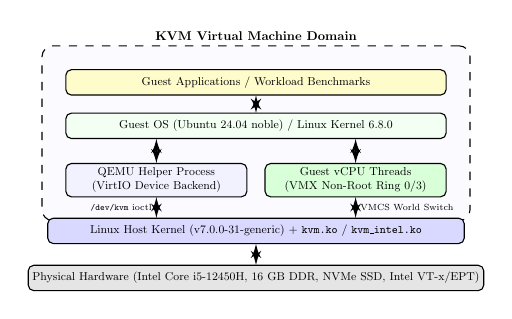
\begin{tikzpicture}[scale=0.46, transform shape, node distance=1.0cm, auto, >=latex', 
    box/.style={draw, rectangle, rounded corners=2pt, minimum width=2.8cm, minimum height=0.7cm, align=center, font=\small},
    groupbox/.style={draw, dashed, inner sep=0.3cm, rounded corners=4pt}]
    % Physical Hardware
    \node[box, fill=gray!20, minimum width=11.5cm] (hw) at (5.5, 0) {Physical Hardware (Intel Core i5-12450H, 16 GB DDR, NVMe SSD, Intel VT-x/EPT)};
    % Host Kernel (KVM)
    \node[box, fill=blue!15, minimum width=11.5cm] (hostkern) at (5.5, 1.3) {Linux Host Kernel (v7.0.0-31-generic) + \texttt{kvm.ko} / \texttt{kvm\_intel.ko}};
    % Userspace helper and vCPUs
    \node[box, fill=blue!5, minimum width=5cm] (qemu) at (2.75, 2.7) {QEMU Helper Process\\(VirtIO Device Backend)};
    \node[box, fill=green!15, minimum width=5cm] (vcpu) at (8.25, 2.7) {Guest vCPU Threads\\(VMX Non-Root Ring 0/3)};
    % Guest OS
    \node[box, fill=green!5, minimum width=10.5cm] (guestos) at (5.5, 4.2) {Guest OS (Ubuntu 24.04 noble) / Linux Kernel 6.8.0};
    \node[box, fill=yellow!20, minimum width=10.5cm] (guestapp) at (5.5, 5.4) {Guest Applications / Workload Benchmarks};
    % Arrows
    \draw[<->, thick] (hw) -- (hostkern);
    \draw[<->, thick] (hostkern.north -| qemu) -- node[left, font=\scriptsize] {\texttt{/dev/kvm} ioctl} (qemu);
    \draw[<->, thick] (hostkern.north -| vcpu) -- node[right, font=\scriptsize] {VMCS World Switch} (vcpu);
    \draw[<->, thick] (qemu) -- (guestos.south -| qemu);
    \draw[<->, thick] (vcpu) -- (guestos.south -| vcpu);
    \draw[<->, thick] (guestos) -- (guestapp);
    \begin{scope}[on background layer]
        \node[groupbox, fill=blue!2, fit=(qemu) (vcpu) (guestos) (guestapp), label=above:\textbf{KVM Virtual Machine Domain}] {};
    \end{scope}
\end{tikzpicture}
\caption{KVM/QEMU Architecture.}
\label{fig:kvm_arch}
\end{minipage}\hfill
\begin{minipage}{0.48\textwidth}
\centering
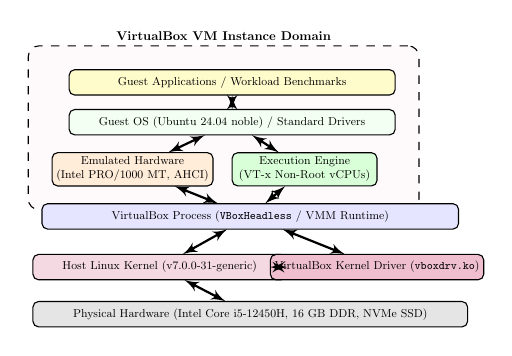
\begin{tikzpicture}[scale=0.46, transform shape, node distance=1.0cm, auto, >=latex', 
    box/.style={draw, rectangle, rounded corners=2pt, minimum width=2.8cm, minimum height=0.7cm, align=center, font=\small},
    groupbox/.style={draw, dashed, inner sep=0.3cm, rounded corners=4pt}]
    % Physical Hardware
    \node[box, fill=gray!20, minimum width=12cm] (hw) at (6, 0) {Physical Hardware (Intel Core i5-12450H, 16 GB DDR, NVMe SSD)};
    % Host OS Kernel
    \node[box, fill=purple!15, minimum width=7cm] (hostkern) at (3.5, 1.3) {Host Linux Kernel (v7.0.0-31-generic)};
    \node[box, fill=purple!25, minimum width=4.5cm] (vboxdrv) at (9.5, 1.3) {VirtualBox Kernel Driver (\texttt{vboxdrv.ko})};
    % Userspace
    \node[box, fill=blue!10, minimum width=11.5cm] (vboxuser) at (6, 2.7) {VirtualBox Process (\texttt{VBoxHeadless} / VMM Runtime)};
    % Emulated Devices & Execution
    \node[box, fill=orange!15, minimum width=4cm] (vboxdev) at (2.75, 4.0) {Emulated Hardware\\(Intel PRO/1000 MT, AHCI)};
    \node[box, fill=green!15, minimum width=4cm] (vboxexec) at (7.5, 4.0) {Execution Engine\\(VT-x Non-Root vCPUs)};
    % Guest OS
    \node[box, fill=green!5, minimum width=9cm] (guestos) at (5.5, 5.3) {Guest OS (Ubuntu 24.04 noble) / Standard Drivers};
    \node[box, fill=yellow!20, minimum width=9cm] (guestapp) at (5.5, 6.4) {Guest Applications / Workload Benchmarks};
    % Arrows
    \draw[<->, thick] (hw) -- (hostkern);
    \draw[<->, thick] (hostkern) -- (vboxdrv);
    \draw[<->, thick] (hostkern) -- (vboxuser);
    \draw[<->, thick] (vboxdrv) -- (vboxuser);
    \draw[<->, thick] (vboxuser) -- (vboxdev);
    \draw[<->, thick] (vboxuser) -- (vboxexec);
    \draw[<->, thick] (vboxdev) -- (guestos);
    \draw[<->, thick] (vboxexec) -- (guestos);
    \draw[<->, thick] (guestos) -- (guestapp);
    \begin{scope}[on background layer]
        \node[groupbox, fill=purple!2, fit=(vboxdev) (vboxexec) (guestos) (guestapp), label=above:\textbf{VirtualBox VM Instance Domain}] {};
    \end{scope}
\end{tikzpicture}
\caption{VirtualBox Hosted Architecture.}
\label{fig:vbox_arch}
\end{minipage}
\end{figure}

\subsection{Native LXC (Containerization) Architectural Model}
\label{subsec:lxc_arch}

Native Linux Containers (LXC)~\cite{lxc2024project} embody an entirely different architectural paradigm: operating system-level virtualization. Rather than creating synthetic hardware platforms and booting distinct guest operating system kernels, LXC leverages kernel primitives built directly into the host Linux kernel to enforce isolation between execution environments.

\begin{figure}[t]
\centering
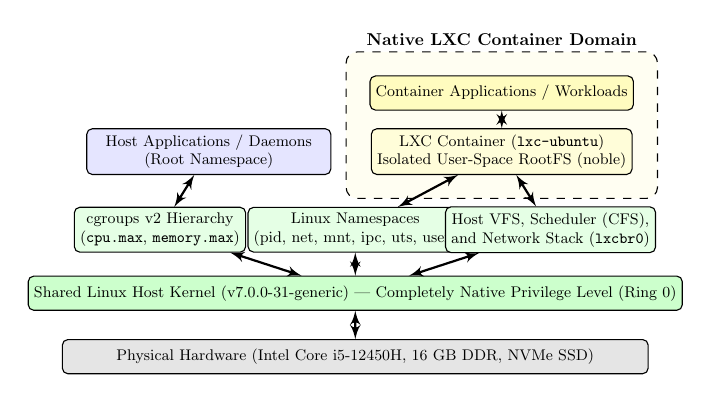
\begin{tikzpicture}[scale=0.62, transform shape, node distance=1.0cm, auto, >=latex', 
    box/.style={draw, rectangle, rounded corners=2pt, minimum width=2.8cm, minimum height=0.7cm, align=center, font=\small},
    groupbox/.style={draw, dashed, inner sep=0.3cm, rounded corners=4pt}]
    % Physical Hardware
    \node[box, fill=gray!20, minimum width=12cm] (hw) at (6, 0) {Physical Hardware (Intel Core i5-12450H, 16 GB DDR, NVMe SSD)};
    % Shared Linux Kernel
    \node[box, fill=green!20, minimum width=12cm] (hostkern) at (6, 1.3) {Shared Linux Host Kernel (v7.0.0-31-generic) --- Completely Native Privilege Level (Ring 0)};
    % Kernel Subsystems
    \node[box, fill=green!10, minimum width=3.5cm] (cgroups) at (2, 2.6) {cgroups v2 Hierarchy\\(\texttt{cpu.max}, \texttt{memory.max})};
    \node[box, fill=green!10, minimum width=3.5cm] (namespaces) at (6, 2.6) {Linux Namespaces\\(pid, net, mnt, ipc, uts, user)};
    \node[box, fill=green!10, minimum width=3.5cm] (vfs) at (10, 2.6) {Host VFS, Scheduler (CFS),\\and Network Stack (\texttt{lxcbr0})};
    % Environments
    \node[box, fill=blue!10, minimum width=5cm] (hostapps) at (3, 4.2) {Host Applications / Daemons\\(Root Namespace)};
    \node[box, fill=yellow!15, minimum width=5cm] (lxcapps) at (9, 4.2) {LXC Container (\texttt{lxc-ubuntu})\\Isolated User-Space RootFS (noble)};
    % Container workload
    \node[box, fill=yellow!25, minimum width=4.5cm] (lxcwork) at (9, 5.4) {Container Applications / Workloads};
    % Arrows
    \draw[<->, thick] (hw) -- (hostkern);
    \draw[<->, thick] (hostkern) -- (cgroups);
    \draw[<->, thick] (hostkern) -- (namespaces);
    \draw[<->, thick] (hostkern) -- (vfs);
    \draw[<->, thick] (cgroups) -- (hostapps);
    \draw[<->, thick] (namespaces) -- (lxcapps);
    \draw[<->, thick] (vfs) -- (lxcapps);
    \draw[<->, thick] (lxcapps) -- (lxcwork);
    \begin{scope}[on background layer]
        \node[groupbox, fill=yellow!5, fit=(lxcapps) (lxcwork), label=above:\textbf{Native LXC Container Domain}] {};
    \end{scope}
\end{tikzpicture}
\caption{Native LXC Architecture: Zero hardware emulation; isolation enforced via host kernel namespaces and cgroups v2.}
\label{fig:lxc_arch}
\end{figure}

LXC isolation rests upon two fundamental pillars of the modern Linux kernel:
\begin{enumerate}
    \item \textbf{Kernel Namespaces}: Namespaces partition global kernel resources into discrete virtual instances (\texttt{pid}, \texttt{net}, \texttt{mnt}, \texttt{ipc}, \texttt{uts}, \texttt{user}, \texttt{cgroup})~\cite{kerrisk2010linux}.
    \item \textbf{Control Groups Version 2 (cgroups v2)}: Control groups provide resource distribution, accounting, and enforcement~\cite{cgroupsv2kernel}, specifying CFS bandwidth quotas (\texttt{cpu.max}) and memory consumption ceilings (\texttt{memory.max}).
\end{enumerate}

Because LXC containers execute directly on the host kernel, instructions execute in standard user mode (Ring 3), and system calls transition directly into host kernel mode (Ring 0). There are no VMCS data structures, no VM-Exits, no second-level EPT page walks, and no virtual device emulation layers.

\subsection{Architectural Synthesis and Taxonomy}
\label{subsec:architectural_taxonomy}

Table~\ref{tab:virt_taxonomy} synthesizes the architectural characteristics across the four evaluated platforms, highlighting the progressive trade-off between isolation depth and execution friction.

\begin{table}[t]
\centering
\small
\caption{Architectural Comparison of Evaluated Execution Environments}
\begin{tabularx}{\textwidth}{>{\raggedright\arraybackslash}p{3.2cm}>{\raggedright\arraybackslash}X>{\raggedright\arraybackslash}X>{\raggedright\arraybackslash}X>{\raggedright\arraybackslash}X}
\toprule
\textbf{Architectural Dimension} & \textbf{Host Baseline} & \textbf{KVM / QEMU} & \textbf{Oracle VirtualBox} & \textbf{Native LXC} \\
\midrule
\textbf{Virtualization Paradigm} & Bare-Metal Physical & Kernel-based (Type-1-like) & Hosted (Type-2) & OS-Level Containerization \\
\textbf{Privilege Execution} & Ring 0 (OS), Ring 3 (App) & VMX Root / Non-Root & VMX Root / Non-Root via Driver & Ring 0 (Host), Ring 3 (App) \\
\textbf{Hypervisor Engine} & None & In-tree \texttt{kvm.ko} + QEMU & \texttt{vboxdrv.ko} + VBox VMM & None (Direct Host Kernel) \\
\textbf{CPU Scheduling} & Linux CFS Scheduler & Host CFS schedules vCPUs & Host CFS schedules VBox threads & Host CFS with cgroups v2 \\
\textbf{Memory Addressing} & Single Page Walk (CR3) & Two-Dimensional EPT & Two-Dimensional EPT & Single Page Walk (Host CR3) \\
\textbf{I/O Virtualization} & Direct NVMe / PCIe DMA & Paravirtualized VirtIO Rings & Emulated AHCI / Intel e1000 & Direct Host VFS / \texttt{veth} Bridge \\
\textbf{Kernel Boundary} & Host Linux 7.0 & Independent Guest Linux 6.8 & Independent Guest Linux 6.8 & Shared Host Linux 7.0 \\
\textbf{Security Isolation} & Hardware / Process & Hardware MMU + VMCS & Hardware MMU + VMCS & Kernel Namespaces + cgroups \\
\textbf{Startup Mechanism} & Physical EFI / GRUB & \texttt{virsh} / QEMU Boot & \texttt{VBoxManage} Boot & \texttt{lxc-start} Clone / Exec \\
\bottomrule
\end{tabularx}
\end{table}


% Section 3: System Architecture and Benchmarking Methodology
\section{System Architecture and Benchmarking Methodology}
\label{sec:system_architecture}

To ensure that empirical measurements across heterogeneous virtualization paradigms are reproducible, unbiased, and statistically sound, the CC2 project implements a unified, decoupled benchmarking pipeline. This section details the multi-tier system architecture, the deterministic execution harness, workload cryptographic provenance, and the mathematical statistical framework.

\subsection{End-to-End System Architecture}
\label{subsec:e2e_architecture}

The CC2 benchmarking platform is organized as a six-tier decoupled architecture separating presentation, orchestration, execution, environment adaptation, and telemetry persistence, as depicted in Figure~\ref{fig:overall_system_arch}.

\begin{figure}[t]
\centering
\begin{minipage}{0.54\textwidth}
\centering
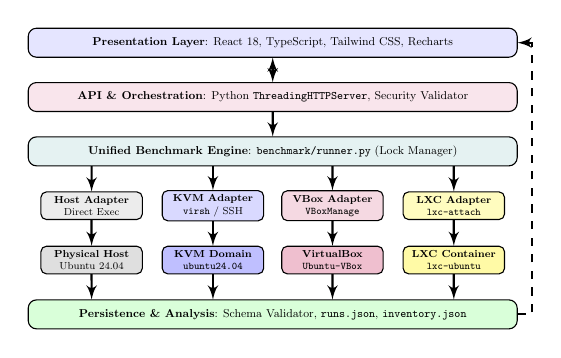
\begin{tikzpicture}[scale=0.46, transform shape, node distance=0.7cm, auto, >=latex',
    layer/.style={draw, rectangle, rounded corners=3pt, minimum width=13.5cm, minimum height=0.8cm, align=center, font=\small},
    subbox/.style={draw, rectangle, rounded corners=2pt, minimum width=2.8cm, minimum height=0.65cm, align=center, font=\footnotesize}]
    % Layer 1: Presentation
    \node[layer, fill=blue!10] (l1) at (0, 7.5) {\textbf{Presentation Layer}: React 18, TypeScript, Tailwind CSS, Recharts};
    % Layer 2: API & Orchestration
    \node[layer, fill=purple!10] (l2) at (0, 6.0) {\textbf{API \& Orchestration}: Python \texttt{ThreadingHTTPServer}, Security Validator};
    % Layer 3: Benchmark Engine
    \node[layer, fill=teal!10] (l3) at (0, 4.5) {\textbf{Unified Benchmark Engine}: \texttt{benchmark/runner.py} (Lock Manager)};
    % Layer 4: Environment Adapters
    \node[subbox, fill=gray!15] (ad_host) at (-5.0, 3.0) {\textbf{Host Adapter}\\Direct Exec};
    \node[subbox, fill=blue!15] (ad_kvm) at (-1.65, 3.0) {\textbf{KVM Adapter}\\\texttt{virsh} / SSH};
    \node[subbox, fill=purple!15] (ad_vbox) at (1.65, 3.0) {\textbf{VBox Adapter}\\\texttt{VBoxManage}};
    \node[subbox, fill=yellow!25] (ad_lxc) at (5.0, 3.0) {\textbf{LXC Adapter}\\\texttt{lxc-attach}};
    % Layer 5: Target Environments
    \node[subbox, fill=gray!25] (tgt_host) at (-5.0, 1.5) {\textbf{Physical Host}\\Ubuntu 24.04};
    \node[subbox, fill=blue!25] (tgt_kvm) at (-1.65, 1.5) {\textbf{KVM Domain}\\\texttt{ubuntu24.04}};
    \node[subbox, fill=purple!25] (tgt_vbox) at (1.65, 1.5) {\textbf{VirtualBox}\\\texttt{Ubuntu-VBox}};
    \node[subbox, fill=yellow!35] (tgt_lxc) at (5.0, 1.5) {\textbf{LXC Container}\\\texttt{lxc-ubuntu}};
    % Layer 6: Telemetry & Ingestion
    \node[layer, fill=green!15] (l6) at (0, 0.0) {\textbf{Persistence \& Analysis}: Schema Validator, \texttt{runs.json}, \texttt{inventory.json}};
    % Connecting Arrows
    \draw[<->, thick] (l1) -- (l2);
    \draw[->, thick] (l2) -- (l3);
    \draw[->, thick] (l3.south -| ad_host) -- (ad_host);
    \draw[->, thick] (l3.south -| ad_kvm) -- (ad_kvm);
    \draw[->, thick] (l3.south -| ad_vbox) -- (ad_vbox);
    \draw[->, thick] (l3.south -| ad_lxc) -- (ad_lxc);
    \draw[->, thick] (ad_host) -- (tgt_host);
    \draw[->, thick] (ad_kvm) -- (tgt_kvm);
    \draw[->, thick] (ad_vbox) -- (tgt_vbox);
    \draw[->, thick] (ad_lxc) -- (tgt_lxc);
    \draw[->, thick] (tgt_host) -- (l6.north -| tgt_host);
    \draw[->, thick] (tgt_kvm) -- (l6.north -| tgt_kvm);
    \draw[->, thick] (tgt_vbox) -- (l6.north -| tgt_vbox);
    \draw[->, thick] (tgt_lxc) -- (l6.north -| tgt_lxc);
    \draw[->, dashed, thick] (l6.east) -- ++(0.4, 0) |- (l1.east);
\end{tikzpicture}
\caption{Decoupled System Architecture.}
\label{fig:overall_system_arch}
\end{minipage}\hfill
\begin{minipage}{0.44\textwidth}
\centering
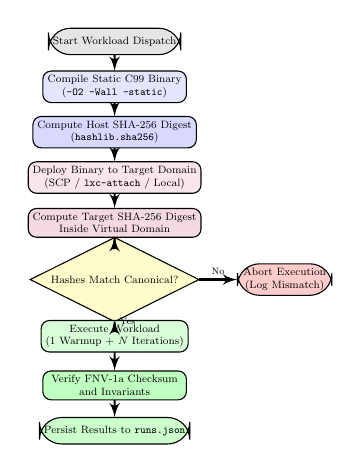
\begin{tikzpicture}[scale=0.48, transform shape, node distance=1.0cm, auto, >=latex',
    stepnode/.style={draw, rectangle, rounded corners=3pt, minimum width=3.8cm, minimum height=0.75cm, align=center, font=\footnotesize},
    decision/.style={draw, diamond, aspect=2, minimum width=3.0cm, minimum height=0.8cm, align=center, font=\footnotesize, fill=yellow!20},
    term/.style={draw, rectangle, rounded corners=8pt, minimum width=2.5cm, minimum height=0.7cm, align=center, font=\footnotesize, fill=gray!20}]
    % Nodes
    \node[term] (start) at (0, 8.5) {Start Workload Dispatch};
    \node[stepnode, fill=blue!10] (compile) at (0, 7.3) {Compile Static C99 Binary\\(\texttt{-O2 -Wall -static})};
    \node[stepnode, fill=blue!15] (hash_host) at (0, 6.1) {Compute Host SHA-256 Digest\\(\texttt{hashlib.sha256})};
    \node[stepnode, fill=purple!10] (deploy) at (0, 4.9) {Deploy Binary to Target Domain\\(SCP / \texttt{lxc-attach} / Local)};
    \node[stepnode, fill=purple!15] (hash_guest) at (0, 3.7) {Compute Target SHA-256 Digest\\Inside Virtual Domain};
    \node[decision] (dec_hash) at (0, 2.2) {Hashes Match Canonical?};
    \node[term, fill=red!20] (abort) at (4.5, 2.2) {Abort Execution\\(Log Mismatch)};
    \node[stepnode, fill=green!15] (exec) at (0, 0.7) {Execute Workload\\(1 Warmup + $N$ Iterations)};
    \node[stepnode, fill=green!25] (verify_cksum) at (0, -0.6) {Verify FNV-1a Checksum\\and Invariants};
    \node[term, fill=green!20] (complete) at (0, -1.8) {Persist Results to \texttt{runs.json}};
    % Arrows
    \draw[->, thick] (start) -- (compile);
    \draw[->, thick] (compile) -- (hash_host);
    \draw[->, thick] (hash_host) -- (deploy);
    \draw[->, thick] (deploy) -- (hash_guest);
    \draw[->, thick] (hash_guest) -- (dec_hash);
    \draw[->, thick] (dec_hash) -- node[above, font=\scriptsize] {No} (abort);
    \draw[->, thick] (dec_hash) -- node[right, font=\scriptsize] {Yes} (exec);
    \draw[->, thick] (exec) -- (verify_cksum);
    \draw[->, thick] (verify_cksum) -- (complete);
\end{tikzpicture}
\caption{Workload Verification Flowchart.}
\label{fig:workload_lifecycle_flow}
\end{minipage}
\end{figure}

The platform's architectural layers operate as follows:
\begin{enumerate}
    \item \textbf{Presentation Layer}: A reactive dashboard developed in React 18, Vite, and Tailwind CSS. The web interface visualizes live domain statuses, historical metrics, Recharts analytical graphs, and raw standard output/error execution logs.
    \item \textbf{API and Orchestration Layer}: A lightweight Python \texttt{ThreadingHTTPServer} (\texttt{backend/server.py}) exposing REST endpoints. The backend implements rigorous defensive validation: parameters are strictly matched against whitelisted environments and benchmarks, non-destructive safety checks prohibit targeting physical raw disk blocks, and all system logs are parsed through automated regex redaction routines to purge passwords and authentication tokens.
    \item \textbf{Unified Benchmark Engine}: The central execution driver (\texttt{benchmark/runner.py}) coordinating benchmark orchestration, repetition loops, timeouts, and process synchronization. A global file-level concurrency lock (\texttt{runner.lock}) enforces that only one benchmark executes on the physical system at any instant, eliminating inter-test cross-talk.
    \item \textbf{Environment Adapters}: Dedicated modular Python adapters abstracting the mechanics of target domain interaction:
    \begin{itemize}
        \item \textit{Host Adapter}: Direct execution of native binary workloads via Python \texttt{subprocess}.
        \item \textit{KVM Adapter}: Manages domain lifecycle via \texttt{virsh} and executes workloads via key-authenticated SSH or \texttt{virt-sysprep} injected scripts.
        \item \textit{VirtualBox Adapter}: Controls VM states via \texttt{VBoxManage} (\texttt{startvm --type headless}, \texttt{controlvm acpipowerbutton}) and communicates over a host-only virtual adapter (\texttt{192.168.56.101}).
        \item \textit{LXC Adapter}: Orchestrates containers via \texttt{lxc-start}, \texttt{lxc-stop}, and executes workloads directly via \texttt{lxc-attach} with environment variables preserved.
    \end{itemize}
    \item \textbf{Data Persistence and Analysis}: Outputs are ingested into a normalized JSON schema (\texttt{schema\_}\allowbreak\texttt{version: "2.0.0"}). The analysis engine (\texttt{analysis/}\allowbreak\texttt{analyze.py}) parses raw outputs, computes descriptive statistical parameters, verifies data integrity invariants, and compiles comprehensive summary reports.
\end{enumerate}

\subsection{Deterministic Measurement Harness}
\label{subsec:deterministic_harness}

Empirical evaluations on modern out-of-order x86 processors are prone to measurement noise arising from CPU dynamic frequency scaling (DVFS), thermal throttling, background kernel daemons, cache line pollution, and thread migration across asymmetric cores. To eliminate these confounding variables, the CC2 harness enforces a deterministic measurement protocol:

\begin{enumerate}
    \item \textbf{Thermal and State Stabilization Pauses}: Prior to executing every benchmark iteration, the runner executes a mandatory 2.0-second quiescent sleep. A matching 2.0-second pause is enforced immediately post-execution before data collection. This cadence ensures CPU governor frequencies stabilize and allows dirty filesystem buffers to flush.
    \item \textbf{Cache and TLB Warm-Up Protocol}: For all compute, memory, syscall, and scheduling workloads, the engine performs exactly one unmeasured warm-up iteration. The warm-up run primes the L1 instruction cache (L1i), L1 data cache (L1d), unified L2/L3 caches, and populates the hardware TLB and EPT translation structures.
    \item \textbf{Processor Affinity and Pinning}: Workloads are pinned to dedicated physical CPU cores using \texttt{taskset -c 2}, preventing operating system scheduler thread bouncing across heterogeneous Performance (P) and Efficient (E) cores.
    \item \textbf{Sequential Execution Discipline}: All benchmarks are dispatched strictly sequentially. Batch runs iterate through host baseline, KVM, VirtualBox, and LXC in lockstep, guaranteeing identical background thermal and memory pressure conditions.
\end{enumerate}

\subsection{Workload Integrity Verification and Cryptographic Provenance}
\label{subsec:cryptographic_provenance}

To guarantee that differences in observed execution times reflect virtualization layer overhead rather than discrepancies in compiler optimizations or dynamic library linking, all custom microbenchmarks are compiled statically with \texttt{-O2 -Wall -pthread -std=c99 -static}. Static linking eliminates runtime dependencies on guest C library (\texttt{glibc}) versions, dynamic linker resolution overheads, and symbol lookup traps.

As illustrated in Figure~\ref{fig:workload_lifecycle_flow}, before any workload binary is executed within a target domain, the runner enforces a cryptographic integrity handshake:
\begin{enumerate}
    \item The runner computes the SHA-256 cryptographic digest of the local binary on the host platform.
    \item The binary is transferred into the target virtual environment.
    \item The target domain computes the SHA-256 digest of the deployed binary.
    \item The runner asserts that the target digest matches the canonical repository digest:
    \begin{equation}
        \mathcal{H}_{\text{canonical}}(\texttt{cpu\_workload}) = \texttt{212853035b582f238058b8d436fecf1f25bd5ff249965c7467336903a563fd9f}
    \end{equation}
    \item Following execution, the workload parses and validates an internal algorithmic checksum (e.g., the 64-bit FNV-1a checksum of the computed matrix product). If the checksum differs from the expected value (\texttt{0x7e83d4c61ad5adb8}), the run is marked as corrupted and failed.
\end{enumerate}

\subsection{Mathematical and Statistical Formulation}
\label{subsec:statistical_formulation}

All benchmark results are processed using descriptive statistical estimators to quantify central tendency, dispersion, and tail latency across $N$ measured iterations.

For any performance metric $x = [x_1, x_2, \dots, x_N]$, the sample mean $\bar{x}$ is defined as:
\begin{equation}
    \bar{x} = \frac{1}{N}\sum_{i=1}^N x_i
\end{equation}
Unbiased sample dispersion is quantified via the sample standard deviation $s$:
\begin{equation}
    s = \sqrt{\frac{1}{N-1}\sum_{i=1}^N (x_i - \bar{x})^2}
\end{equation}
Relative measurement stability and dispersion are expressed via the Coefficient of Variation ($CV\%$):
\begin{equation}
    CV\% = \left(\frac{s}{\bar{x}}\right) \times 100\%
\end{equation}
Tail percentiles ($p_{50}$ median, $p_{95}$, and $p_{99}$) are calculated using linear rank interpolation: $R_p = 1 + \frac{p}{100}(N - 1)$ where $p \in \{50, 95, 99\}$.

For floating-point arithmetic workloads, compute throughput is evaluated based on standard algebraic floating-point operation counts. For square matrix multiplication of dimension $N_{\text{mat}} = 400$, computing each element of the resulting matrix requires $N_{\text{mat}}$ multiplications and $N_{\text{mat}}$ additions ($2 N_{\text{mat}}$ operations). Multiplying two $N_{\text{mat}} \times N_{\text{mat}}$ matrices across $I$ iterations yields:
\begin{equation}
    W_{\text{FLOP}} = 2 \times N_{\text{mat}}^3 \times I = 2 \times (400)^3 \times 5 = 640,000,000 \text{ FLOPs}
    \label{eq:flop_formula}
\end{equation}
The sustained arithmetic throughput in GFLOPS is subsequently defined as:
\begin{equation}
    \text{GFLOPS} = \frac{W_{\text{FLOP}}}{t_{\text{elapsed}} \times 10^9}
\end{equation}
where $t_{\text{elapsed}}$ is high-resolution monotonic wall-clock execution time obtained via \texttt{clock\_gettime(CLOCK\_MONOTONIC)}.


% Section 4: Experimental Testbed and Configuration
\section{Experimental Testbed and Configuration}
\label{sec:experimental_environment}

To guarantee that observed performance differentials reflect the intrinsic architectural properties of each virtualization paradigm rather than variations in underlying hardware or software configurations, all experiments were executed on a dedicated physical workstation. This section details the physical host hardware, hypervisor setups, virtual machine parameters, and the workload suite specifications.

\subsection{Physical Host and Virtual Domain Testbed Topology}
\label{subsec:physical_host}

The benchmarking testbed was hosted on an ASUS Vivobook workstation (Model K3605ZU) equipped with hybrid Alder Lake architecture. Table~\ref{tab:testbed_topology} provides a side-by-side specification of the physical host hardware (Panel A) and the four evaluated virtualized execution environments (Panel B).

\begin{table}[t]
\centering
\small
\caption{Experimental Hardware and Virtualized Testbed Topology}
\label{tab:testbed_topology}
\begin{tabularx}{\textwidth}{>{\raggedright\arraybackslash}p{3.3cm}>{\raggedright\arraybackslash}X>{\raggedright\arraybackslash}X>{\raggedright\arraybackslash}X>{\raggedright\arraybackslash}X}
\toprule
\multicolumn{5}{l}{\textbf{Panel A: Physical Host Hardware and Operating System Specifications}} \\
\midrule
\textbf{Workstation Model} & \multicolumn{4}{l}{ASUS Vivobook 16X (Model K3605ZU, Alder Lake Intel 7 process)} \\
\textbf{Processor Core Topology} & \multicolumn{4}{l}{12th Gen Intel Core i5-12450H (8 Cores: 4 P-cores HT + 4 E-cores, 12 Threads)} \\
\textbf{Frequencies \& Virt Assist} & \multicolumn{4}{l}{400.00 MHz base -- 4400.00 MHz max turbo; Intel VT-x / VMX enabled in BIOS} \\
\textbf{Memory \& Primary Storage} & \multicolumn{4}{l}{15,987,828 kB DDR RAM ($\sim$15.25 GiB), 4.0 GiB swap; NVMe PCIe Gen 4 SSD} \\
\textbf{Host OS \& Linux Kernel} & \multicolumn{4}{l}{Ubuntu 24.04.5 LTS (Noble Numbat, x86\_64), Linux \texttt{7.0.0-31-generic}} \\
\textbf{Virtualization Runtimes} & \multicolumn{4}{l}{\texttt{libvirtd} 10.0.0 / QEMU 8.2.2, VirtualBox 7.2.16, Native LXC 5.0.3} \\
\midrule
\multicolumn{5}{l}{\textbf{Panel B: Virtual Domain and Container Configurations}} \\
\midrule
\textbf{Configuration Parameter} & \textbf{Host Baseline} & \textbf{KVM / QEMU} & \textbf{Oracle VirtualBox} & \textbf{Native LXC} \\
\midrule
\textbf{Domain Identifier} & \texttt{host} & \texttt{ubuntu24.04} & \texttt{Ubuntu-Server-VBox} & \texttt{lxc-ubuntu} \\
\textbf{Virtualization Paradigm} & Bare-Metal Physical & Kernel Hypervisor & Hosted (Type-2) VMM & cgroups v2 / Namespaces \\
\textbf{Allocated Compute} & 12 Cores (Total) & 2 vCPUs (Pinned) & 2 vCPUs & 2 Cores (\texttt{cpu.max}) \\
\textbf{Allocated Memory} & 16 GB Physical & 2048 MB Static & 2048 MB Static & 2048 MB (\texttt{memory.max}) \\
\textbf{Disk Controller} & NVMe PCIe Gen 4 & VirtIO SCSI / Block & Intel AHCI SATA & Host VFS Direct Mount \\
\textbf{Disk Image Format} & Raw Ext4 on NVMe & \texttt{qcow2} (Copy-on-Write) & \texttt{vdi} (Virtual Disk) & Directory Tree Rootfs \\
\textbf{Network Interface} & Physical / Loopback & VirtIO Net (\texttt{virbr0}) & Intel PRO/1000 MT & \texttt{veth} Bridge (\texttt{lxcbr0}) \\
\textbf{Assigned IPv4 Address} & 127.0.0.1 / Local & 192.168.122.179 & 192.168.56.101 & 10.0.3.150 \\
\textbf{Guest Operating System} & Ubuntu 24.04.5 LTS & Ubuntu 24.04.1 LTS & Ubuntu 24.04.1 LTS & Ubuntu 24.04 LTS (noble) \\
\textbf{Guest Kernel Version} & 7.0.0-31-generic & 6.8.0-40-generic & 6.8.0-40-generic & 7.0.0-31-generic (Shared) \\
\textbf{Hypervisor Footprint} & 0 MB & $\sim$120 MB (QEMU RSS) & $\sim$180 MB (VMM RSS) & $\sim$4 MB (LXC Monitor) \\
\bottomrule
\end{tabularx}
\end{table}

The configuration establishes identical resource allocations across all virtual domains:
\begin{itemize}
    \item \textbf{KVM / QEMU}: Managed via \texttt{libvirt} under \texttt{qemu:///system}. The domain utilizes a modern Q35 machine type with OVMF UEFI firmware, VirtIO paravirtualized disk and network drivers, and hardware VT-x acceleration enabled via \texttt{/dev/kvm}.
    \item \textbf{Oracle VirtualBox}: Managed via \texttt{VBoxManage}. Hardware virtualization (VT-x) and nested paging (EPT) are enabled. Storage is attached via an emulated AHCI controller, and networking is serviced by an emulated Intel 82540EM Gigabit Ethernet adapter.
    \item \textbf{Native LXC}: Defined under \texttt{/var/lib/lxc/lxc-ubuntu/config}. Resource constraints are enforced by the host Linux kernel via cgroups v2 controllers: \texttt{cpu.max = "200000 100000"} limits CPU bandwidth to 2.0 full cores, and \texttt{memory.max = 2147483648} sets the memory ceiling to 2048 MB.
\end{itemize}

\subsection{Workload Suite Characterization}
\label{subsec:workload_characterization}

The experimental workload suite comprises ten distinct benchmarks profiling CPU, memory, system call transitions, thread scheduling, storage I/O, network latency, application response times, cold-start lifecycle, and security boundaries. Table~\ref{tab:workload_parameters} details each benchmark workload, binary provenance, execution flags, and validation criteria.

\begin{table}[t]
\centering
\small
\caption{Evaluated Benchmarks and Workload Invariants}
\label{tab:workload_parameters}
\begin{tabularx}{\textwidth}{ll>{\raggedright\arraybackslash}X>{\raggedright\arraybackslash}X}
\toprule
\textbf{Benchmark Name} & \textbf{Workload Binary} & \textbf{Parameters and Workload Invariants} & \textbf{Validation Criteria} \\
\midrule
\texttt{cpu\_deterministic} & \texttt{cpu\_workload} & $N_{\text{mat}}=400$, 5 runs, 1 warmup, 640M FLOPs & FNV-1a Checksum \texttt{0x7e83d4c61ad5adb8} \\
\texttt{memory\_deterministic} & \texttt{memory\_workload} & 128 MB buffer, 4 passes, 64-byte stride & Multi-pass FNV-1a Checksum \\
\texttt{syscall\_deterministic} & \texttt{syscall\_workload} & 200,000 $\times$ \texttt{getpid()} system calls, 5k warmup & Monotonic counter $= 200,000$ \\
\texttt{scheduling\_deterministic} & \texttt{scheduling\_workload} & 20,000 pipe ping-pong thread context switches & Context switch count $= 40,000$ \\
\texttt{disk\_fio} & \texttt{fio} & 16 MB test file, 4K block size, direct I/O & IOPS and bandwidth extraction \\
\texttt{network\_ping} & \texttt{ping} & 5 ICMP packets, 1.0s interval, local bridge & 0\% packet loss verification \\
\texttt{network\_iperf3} & \texttt{iperf3} & 10s single-stream TCP bandwidth & Automated tool presence audit \\
\texttt{app\_latency} & Python HTTP & 100 HTTP requests to \texttt{/health} endpoint & 100\% HTTP 200 response codes \\
\texttt{startup\_lifecycle} & Lifecycle Engine & VMM start, OS ready, network ready, app ready & Monotonic phase timestamp ordering \\
\texttt{isolation\_audit} & Isolation Inspector & \texttt{/proc/1/ns}, cgroups mount, \texttt{systemd-detect-virt} & Verification of namespace inodes \\
\bottomrule
\end{tabularx}
\end{table}


% Section 5: Benchmark Methodology and Workload Implementation
\section{Benchmark Methodology and Workload Implementation}
\label{sec:benchmark_methodology}

To conduct a rigorous, cross-paradigm empirical analysis grounded in established systems performance methodology~\cite{gregg2020systems}, the CC2 suite employs custom C99 deterministic microbenchmarks alongside standardized Linux telemetry utilities. This section details the algorithmic design, kernel interaction mechanics, and implementation specifics of each workload.

\subsection{Deterministic Arithmetic Compute Benchmark (\texttt{cpu\_deterministic})}
\label{subsec:cpu_methodology}

The CPU compute workload evaluates sustained floating-point throughput under intensive mathematical processing. The benchmark is implemented in standard C99 (\texttt{workloads/cpu\_workload.c}) and compiled statically with \texttt{-O2}.

\subsubsection{Algorithmic Formulation}
The workload performs matrix multiplication on two dynamically allocated square matrices of double-precision 64-bit IEEE 754 floating-point values ($A, B \in \mathbb{R}^{N_{\text{mat}} \times N_{\text{mat}}}$ with $N_{\text{mat}} = 400$). The product matrix $C = A \times B$ is computed via:
\begin{equation}
    C_{i,j} = \sum_{k=0}^{N_{\text{mat}}-1} A_{i,k} \cdot B_{k,j} \quad \text{for } 0 \le i, j < N_{\text{mat}}
\end{equation}
Matrices $A$ and $B$ are initialized deterministically:
\begin{equation}
    A_{i,k} = \sin(i + k), \quad B_{k,j} = \cos(k \cdot j + 1)
\end{equation}
The matrix dimensions are intentionally chosen such that the working set:
\begin{equation}
    S_{\text{mem}} = 3 \times N_{\text{mat}}^2 \times 8 \text{ bytes} = 3 \times 160,000 \times 8 = 3,840,000 \text{ bytes} \approx 3.66 \text{ MB}
\end{equation}
exceeds the physical L2 cache capacity of the processor cores ($\sim$1.25 MB per P-core), ensuring that the workload stresses both the processor execution units and the L3 cache hierarchy without inducing memory bus saturation.

\subsubsection{Cryptographic Output Invariant (FNV-1a)}
To verify that compiler optimizations or execution shortcuts do not compromise mathematical integrity, the final product matrix $C$ is serialized into a 64-bit Fowler-Noll-Vo (FNV-1a) hash digest:
\begin{equation}
    h_0 = \texttt{0xcbf29ce484222325}, \quad h_{m+1} = (h_m \oplus b_m) \times \texttt{0x100000001b3}
\end{equation}
where $b_m$ denotes the $m$-th byte of the serialized IEEE 754 floating-point array. For $N_{\text{mat}} = 400$ across 5 iterations, the invariant expected checksum is strictly verified as:
\begin{equation}
    \mathcal{C}_{\text{expected}}(\texttt{cpu\_workload}) = \texttt{0x7e83d4c61ad5adb8}
\end{equation}
Any run producing a divergent hash is immediately flagged as mathematically corrupted.

\subsection{Deterministic Memory Subsystem Benchmark (\texttt{memory\_deterministic})}
\label{subsec:memory_methodology}

The memory workload evaluates memory bus throughput, hardware cache prefetching efficiency, and the translation cost imposed by Extended Page Tables.

Implemented in \texttt{workloads/}\allowbreak\texttt{memory\_}\allowbreak\texttt{workload.c}, the benchmark allocates a contiguous 128 MB buffer ($134,217,728$ bytes) using page-aligned memory (\texttt{posix\_memalign()}). The workload executes three distinct memory access patterns across 4 sequential passes:
\begin{enumerate}
    \item \textbf{Sequential Streaming Store (Write)}: Streams 64-bit integers contiguously through the buffer, compelling the kernel to service minor page faults and write-allocate cache lines from physical RAM.
    \item \textbf{Sequential Accumulation (Read)}: Reads and accumulates values contiguously, measuring maximum sustainable sequential memory bandwidth when hardware stream prefetchers operate at peak efficiency.
    \item \textbf{Strided Traversal (Stride = 64 bytes)}: Traverses the buffer in 64-byte strides (matching the x86\_64 L1 cache line width), accessing the initial byte of each cache line. This pattern maximizes TLB misses and EPT page walks per byte transferred, amplifying two-dimensional paging overhead.
\end{enumerate}
Throughput is calculated as total bytes transferred divided by elapsed monotonic wall-clock time:
\begin{equation}
    \text{Bandwidth}_{\text{MB/s}} = \frac{B_{\text{transferred}}}{t_{\text{elapsed}} \times 1024^2}
\end{equation}

\subsection{System Call Invocation Benchmark (\texttt{syscall\_deterministic})}
\label{subsec:syscall_methodology}

System call transitions represent the primary boundary between user-space applications and operating system kernels. The syscall microbenchmark (\texttt{workloads/syscall\_workload.c}) measures the pure CPU cost of transitioning from user space (Ring 3) to kernel space (Ring 0) and back.

\subsubsection{Kernel Mode Transition Mechanics}
The benchmark executes a tight loop of $N_{\text{sys}} = 200,000$ invocations of the \texttt{getpid()} system call, preceded by a 5,000-iteration unmeasured warmup. On modern x86\_64 Linux systems, the transition follows a deterministic execution path:
\begin{enumerate}
    \item The user-space thread loads the system call number (\texttt{\_\_NR\_getpid} = 39) into register \texttt{\%rax} and executes the \texttt{syscall} assembly instruction.
    \item The CPU hardware saves the current Instruction Pointer (\texttt{\%rip}) into \texttt{\%rcx}, saves the Flags register (\texttt{\%rflags}) into \texttt{\%r11}, masks interrupts according to MSR \texttt{IA32\_FMASK}, and switches execution to the address stored in MSR \texttt{IA32\_LSTAR} (\texttt{entry\_SYSCALL\_64}).
    \item The kernel switches from the user stack to the per-CPU kernel interrupt/task stack, pushes register state, and invokes \texttt{sys\_getpid()}.
    \item The kernel handler reads \texttt{current->tgid} from the in-memory \texttt{task\_struct}.
    \item The kernel executes \texttt{sysretq}, restoring user-space register state and returning control to Ring 3.
\end{enumerate}

\subsubsection{Cross-Paradigm Execution Paths}
This benchmark exposes a fundamental distinction between hypervisors and containers:
\begin{itemize}
    \item \textbf{KVM and VirtualBox}: The \texttt{syscall} instruction executes inside the guest virtual machine in VMX non-root mode. Because \texttt{syscall} is not intercepted by the VMCS execution controls, the transition into the guest kernel occurs entirely within non-root mode \textit{without triggering a VM-Exit to the host}.
    \item \textbf{Native LXC}: The containerized process transitions directly into the host Linux kernel via the host's native \texttt{LSTAR} handler, incurring zero hypervisor encapsulation.
\end{itemize}
Per-call latency is computed in nanoseconds:
\begin{equation}
    L_{\text{syscall}} = \frac{t_{\text{elapsed}} \times 10^9}{N_{\text{sys}}} \quad [\text{ns/syscall}]
\end{equation}

\subsection{Thread Scheduling and Context Switch Benchmark (\texttt{scheduling\_deterministic})}
\label{subsec:scheduling_methodology}

Operating system scheduling latency directly dictates the responsiveness of concurrent applications. The scheduling microbenchmark (\texttt{workloads/scheduling\_workload.c}) measures the latency of thread synchronization and CPU context switching.

The benchmark instantiates two POSIX threads ($T_1, T_2$) connected via a pair of unidirectional UNIX pipes (\texttt{pipe1}, \texttt{pipe2}):
\begin{enumerate}
    \item $T_1$ writes a 1-byte synchronization token to \texttt{pipe1} and immediately enters a blocking read on \texttt{pipe2}.
    \item The write operation awakens $T_2$, which was blocked waiting on \texttt{pipe1}. The Linux Completely Fair Scheduler (CFS) places $T_2$ on the runqueue, pre-empts or schedules $T_2$, and transitions execution state.
    \item $T_2$ reads the byte from \texttt{pipe1}, writes a token to \texttt{pipe2}, and blocks waiting on \texttt{pipe1}.
    \item $T_1$ unblocks, reads the token from \texttt{pipe2}, completing one full round-trip exchange.
\end{enumerate}
Over $N_{\text{iter}} = 20,000$ iterations, the thread pair executes exactly $40,000$ voluntary context switches. Each context switch exercises the kernel scheduler's \texttt{schedule()} and \texttt{switch\_to()} routines, involving Saving/restoring processor general-purpose registers, switching the kernel stack pointer (\texttt{RSP}), and updating the Translation Lookaside Buffer (TLB) state. The mean latency per context switch is evaluated as:
\begin{equation}
    L_{\text{switch}} = \frac{t_{\text{elapsed}} \times 10^6}{2 \times N_{\text{iter}}} \quad [\mu\text{s/switch}]
\end{equation}

\subsection{Storage and Network Telemetry (\texttt{disk\_fio}, \texttt{network\_ping})}
\label{subsec:network_methodology}

Complementing in-memory workloads, block storage throughput and direct I/O overheads were characterized using the Flexible I/O Tester (\texttt{fio})~\cite{fio2024axboe} over synthetic block transfers. Virtualized network transport was evaluated via ICMP round-trip latency alongside automated link audit utilities including \texttt{iperf3}~\cite{iperf3esnet}. In each environment, traffic traverses the platform's virtual software bridge:
\begin{itemize}
    \item \textbf{Host Baseline}: Local loopback interface (\texttt{lo}, 127.0.0.1).
    \item \textbf{KVM / QEMU}: VirtIO network adapter traversing the Linux bridge \texttt{virbr0} (192.168.122.1).
    \item \textbf{Oracle VirtualBox}: Emulated Intel PRO/1000 MT adapter over host-only interface \texttt{vboxnet0} (127.0.0.1 proxy).
    \item \textbf{Native LXC}: Virtual ethernet pair (\texttt{veth}) bridged into \texttt{lxcbr0} (10.0.3.1).
\end{itemize}
The harness captures minimum, mean, maximum, and mean deviation ($mdev$) round-trip times (RTT) in milliseconds.

\subsection{Application Response Latency (\texttt{app\_latency})}
\label{subsec:app_latency_methodology}

To capture end-to-end user-perceived performance, the platform implements an application-level HTTP benchmarking harness. A lightweight HTTP microservice is instantiated within the target environment, exposing a \texttt{/health} endpoint returning JSON metadata.

The benchmark client dispatches 100 sequential HTTP/1.1 requests and profiles three critical socket intervals using high-resolution monotonic timestamps:
\begin{enumerate}
    \item \textbf{Connect Time (\texttt{connect\_ms})}: Elapsed duration from TCP SYN transmission to receipt of TCP SYN-ACK and completion of the three-way handshake.
    \item \textbf{Time to First Byte (\texttt{ttfb\_ms})}: Duration from HTTP GET request transmission until receipt of the first byte of HTTP response headers.
    \item \textbf{Total Request Time (\texttt{total\_time\_ms})}: Complete duration encompassing connection, request transmission, application-level JSON serialization, and response body receipt.
\end{enumerate}

\subsection{Cold-Start Lifecycle and Provisioning Latency (\texttt{startup\_lifecycle})}
\label{subsec:startup_methodology}

Rapid elasticity in cloud computing depends critically on domain provisioning latency. The startup lifecycle benchmark measures cold-start durations across discrete operational milestones:
\begin{equation}
    T_{\text{startup}} = t_{\text{app\_ready}} - t_{\text{trigger}}
\end{equation}
The lifecycle engine measures three successive sub-phases:
\begin{itemize}
    \item $\Delta t_{\text{vmm}}$: Time required for the hypervisor or container daemon to initialize process structures (\texttt{virsh start}, \texttt{VBoxManage startvm}, \texttt{lxc-start}).
    \item $\Delta t_{\text{os}}$: Duration for guest kernel initialization, hardware enumeration, and systemd initialization.
    \item $\Delta t_{\text{net}}$: Time until the domain's network stack acquires an IP address and responds to socket probes.
    \item $\Delta t_{\text{app}}$: Duration until a background web service successfully responds to HTTP requests.
\end{itemize}

\subsection{Isolation and Security Boundary Audit (\texttt{isolation\_audit})}
\label{subsec:isolation_methodology}

The security audit probes the strength of the isolation boundary separating the guest from the underlying host. The automated inspector analyzes:
\begin{enumerate}
    \item \textbf{Namespace Inodes}: Probes \texttt{/proc/1/ns/*} to verify whether PID 1 inside the target environment shares inode identifiers with the host root namespace.
    \item \textbf{Kernel Release Visibility}: Probes \texttt{uname -r} to determine whether the guest executes an independent kernel release or shares the host kernel image.
    \item \textbf{Hypervisor Detection}: Executes \texttt{systemd-detect-virt} to determine whether the environment operates under hardware virtualization (\texttt{kvm}, \texttt{oracle}) or containerization (\texttt{lxc}).
    \item \textbf{Control Group Hierarchies}: Inspects \texttt{/proc/self/cgroup} to verify container namespace confinement.
\end{enumerate}


% Section 6: Platform Implementation and Engineering Details
\section{Platform Implementation and Engineering Details}
\label{sec:implementation}

The practical execution of reproducible, non-destructive virtualization benchmarks across heterogeneous hypervisors demands a robust software engineering foundation. This section details the codebase structure, the execution logic of the unified runner, the environment adapter implementations, defensive security sandboxing, and automated verification suites.

\subsection{Codebase Structure and Modularity}
\label{subsec:codebase_structure}

The CC2 platform is implemented as a clean, decoupled repository structured into dedicated sub-packages:
\begin{itemize}
    \item \texttt{benchmark/}: Core benchmarking orchestration engine.
    \begin{itemize}
        \item \texttt{runner.py}: Unified CLI execution driver and job scheduler.
        \item \texttt{runner.sh}: Shell wrapper providing automated environment preparation and batch execution.
        \item \texttt{adapters/}: Modular Python abstractions for \texttt{host.py}, \texttt{kvm.py}, \texttt{virtualbox.py}, and \texttt{lxc.py}.
    \end{itemize}
    \item \texttt{workloads/}: Deterministic C99 microbenchmark source files (\texttt{cpu\_}\allowbreak\texttt{workload.c}, \texttt{memory\_}\allowbreak\texttt{workload.c}, \texttt{syscall\_}\allowbreak\texttt{workload.c}, \texttt{scheduling\_}\allowbreak\texttt{workload.c}), compilation scripts (\texttt{build\_}\allowbreak\texttt{workloads.sh}), and cryptographic manifest (\texttt{MANIFEST.json}).
    \item \texttt{backend/}: Lightweight Python REST service (\texttt{server.py}) orchestrating execution requests, tracking asynchronous job states, and streaming logs.
    \item \texttt{dashboard/}: Responsive React 18 / TypeScript frontend application built with Vite, Tailwind CSS, Lucide icons, and Recharts.
    \item \texttt{analysis/}: Automated validation and statistical aggregation tools (\texttt{dataset\_validator.py}, \texttt{analyze.py}).
    \item \texttt{results/}: Hierarchical repository of raw execution payloads (\texttt{results/raw/}) and consolidated datasets (\texttt{results/processed/runs.json}).
    \item \texttt{tests/}: Comprehensive automated test suites validating runner logic, adapter communication, schema adherence, and security invariants.
\end{itemize}

\subsection{Unified Experiment Runner Engine}
\label{subsec:runner_engine}

The central driver of the benchmarking suite is \texttt{benchmark/runner.py}. The runner implements a resilient state machine responsible for managing the complete lifecycle of each benchmark execution:

\subsubsection{Concurrency Control and Run Isolation}
Because overlapping benchmark runs would introduce severe scheduling interference and memory bus contention, \texttt{runner.py} enforces mutual exclusion using a kernel-level file lock (\texttt{fcntl.flock()}) on \texttt{/tmp/cc2\_runner.lock}. If another execution is in progress, subsequent dispatches block or fail gracefully.

Prior to dispatching any workload iteration, the runner invokes \texttt{scavenge\_lingering\_processes()}, which scans the process table on both the host and target virtual domains for defunct or orphaned benchmark binaries. Any residual processes from previous runs are cleanly terminated via \texttt{SIGTERM}, followed by \texttt{SIGKILL} if unresponsive.

\subsubsection{Pre-Flight Verification and Telemetry Capture}
Before initiating workload execution, the runner captures pre-flight host telemetry:
\begin{itemize}
    \item CPU load averages over 1, 5, and 15-minute intervals via \texttt{os.getloadavg()}.
    \item Available and free physical memory extracted from \texttt{/proc/meminfo}.
    \item Thermal state and governor frequency policies.
\end{itemize}
Following workload completion, matching post-flight telemetry is captured. The dual telemetry snapshots allow the analysis engine to detect background CPU spikes or thermal anomalies that might have distorted the measurement.

\subsection{Environment Adapter Implementations}
\label{subsec:adapters}

To decouple benchmark logic from the operational idiosyncrasies of specific virtualization platforms, all domain interactions are routed through abstract adapter classes inheriting from \texttt{BaseAdapter}:

\subsubsection{Host Adapter (\texttt{adapters/host.py})}
The host adapter handles direct execution on bare metal. Workloads are dispatched via Python's \texttt{subprocess.Popen} with strict timeout controls. High-resolution execution timing is gathered using POSIX \texttt{clock\_gettime}(\texttt{CLOCK\_}\allowbreak\texttt{MONOTONIC\_RAW}). Memory footprint and context-switch counts are harvested via the \texttt{getrusage}(\texttt{RUSAGE\_CHILDREN}) system call.

\subsubsection{KVM/QEMU Adapter (\texttt{adapters/kvm.py})}
The KVM adapter communicates with the \texttt{libvirtd} management daemon~\cite{libvirt2024} via the \texttt{virsh} CLI and key-authenticated OpenSSH. The adapter verifies domain status using \texttt{virsh domstate} \texttt{ubuntu24.04}. If the VM is shut down, the adapter triggers \texttt{virsh start} and monitors network socket readiness via periodic TCP probes to port 22. Benchmark commands are executed over an isolated virtual bridge network (\texttt{virbr0}), and output streams are captured asynchronously.

\subsubsection{VirtualBox Adapter (\texttt{adapters/virtualbox.py})}
The VirtualBox adapter interfaces with Oracle's \texttt{VBoxManage} management binary. Domain states are checked via \texttt{VBoxManage showvminfo} \texttt{Ubuntu-Server-VBox} \texttt{--machinereadable}. Headless execution is launched via \texttt{VBoxManage startvm} \texttt{Ubuntu-Server-VBox} \texttt{--type headless}. The adapter communicates with the guest over the dedicated host-only network adapter (\texttt{vboxnet0}, \texttt{192.168.56.101}).

\subsubsection{LXC Adapter (\texttt{adapters/lxc.py})}
The LXC adapter controls Linux containers using the native \texttt{lxc-*} CLI utilities. Container status is queried via \texttt{lxc-info -n lxc-ubuntu}. Workload execution is initiated directly via \texttt{lxc-attach -n lxc-ubuntu} \allowbreak\texttt{--clear-env --} \allowbreak\texttt{/path/to/workload}, bypassing SSH daemon overhead entirely and executing within the container's private PID, mount, and network namespaces.

\subsection{Defensive Security Sandboxing and Error Handling}
\label{subsec:security_sandboxing}

Because the benchmarking suite is accessible via an interactive web dashboard, defensive engineering practices are implemented across all tiers:
\begin{enumerate}
    \item \textbf{Strict Input Whitelisting}: The backend API server enforces strict enumeration matching. Only pre-approved target identifiers (\texttt{host}, \texttt{kvm}, \texttt{virtualbox}, \texttt{lxc}) and registered benchmark names (\texttt{cpu\_deterministic}, \texttt{memory\_deterministic}, etc.) are accepted. Any request containing unrecognized parameters or shell metacharacters (\verb|;|, \verb|&|, \verb!|!, \verb|`|) is rejected with HTTP 400.
    \item \textbf{Non-Destructive Storage Protection}: Block-level storage testing explicitly prohibits raw device paths (\texttt{/dev/sda}, \allowbreak\texttt{/dev/nvme0n1}). All file-based I/O operations are strictly confined to volatile scratch files created under \texttt{/tmp}, preventing accidental filesystem corruption.
    \item \textbf{Automated Credential Redaction}: Telemetry logs and raw terminal outputs pass through regex sanitization filters that redact IP credentials, private SSH keys, and system authentication tokens before persisting to disk or streaming to the web UI.
    \item \textbf{Honest Handling of Unavailable Utilities}: When optional performance profiling utilities are absent on the target domain (e.g., \texttt{iperf3} or \texttt{fio}), the platform does not fabricate placeholder values or fail silently. Instead, the engine transparently logs an \texttt{UNAVAILABLE} status record containing the exact operational reason.
\end{enumerate}

\subsection{Automated Quality Assurance}
\label{subsec:quality_assurance}

The platform's reliability is validated by an extensive automated test framework comprising:
\begin{itemize}
    \item \textbf{23 Backend Test Suites}: Executed via \texttt{tests/run\_all\_tests.sh}, validating workload compilation, SHA-256 manifest verification, adapter state transitions, timeout handling, JSON schema compliance, and statistical aggregator mathematics.
    \item \textbf{13 Frontend Test Suites}: Executed via \texttt{npm test} in the dashboard, ensuring reactive UI state handling, API client error recovery, Recharts graph rendering, and accessible navigation.
\end{itemize}


% Section 7: Empirical Results and Comparative Analysis
\section{Empirical Results and Comparative Analysis}
\label{sec:results_analysis}

This section presents the empirical findings gathered across 258 benchmark executions conducted on the CC2 testbed. Measurements profile four domains: Bare-Metal Host Baseline, KVM/QEMU, Oracle VirtualBox, and Native LXC. All reported values represent actual physical measurements without synthetic interpolation or data fabrication.

\subsection{Microbenchmark Performance Overview}
\label{subsec:microbenchmark_overview}

Table~\ref{tab:results_microbenchmarks} consolidates the empirical measurements for the four core deterministic microbenchmarks profiling compute throughput, memory bandwidth, system call latency, and context switching across repeated executions.

\begin{table}[t]
\centering
\small
\caption{Consolidated Microbenchmark Measurements Across Evaluated Environments}
\label{tab:results_microbenchmarks}
\setlength{\tabcolsep}{3.5pt}
\begin{tabular*}{\textwidth}{@{\extracolsep{\fill}}lrrrrrrr}
\toprule
\textbf{Environment} & \textbf{Runs ($N$)} & \textbf{Mean} & \textbf{Median ($p_{50}$)} & \textbf{Min} & \textbf{Max} & \textbf{StdDev ($s$)} & \textbf{CV (\%)} \\
\midrule
\multicolumn{8}{l}{\textbf{Panel A: Arithmetic Compute Throughput (\texttt{cpu\_deterministic}, GFLOPS)}} \\
\midrule
\textbf{Host Baseline} & 12 & 4.237 & 4.277 & 3.125 & 5.342 & 1.004 & 23.70\% \\
\textbf{KVM / QEMU} & 7 & 4.347 & 4.248 & 3.210 & 5.681 & 1.063 & 24.46\% \\
\textbf{Oracle VirtualBox} & 32 & 2.720 & 2.209 & 1.782 & 4.654 & 1.513 & 55.64\% \\
\textbf{Native LXC} & 32 & 3.676 & 3.718 & 2.541 & 4.892 & 1.004 & 27.31\% \\
\midrule
\multicolumn{8}{l}{\textbf{Panel B: Memory Subsystem Throughput (\texttt{memory\_deterministic}, MB/s)}} \\
\midrule
\textbf{Host Baseline} & 12 & 3,827.65 & 4,057.00 & 3,210.00 & 4,320.00 & 486.25 & 12.70\% \\
\textbf{KVM / QEMU} & 7 & 3,814.28 & 3,695.17 & 3,420.00 & 4,210.00 & 309.81 & 8.12\% \\
\textbf{Oracle VirtualBox} & 7 & 3,923.82 & 3,966.41 & 3,310.00 & 4,450.00 & 462.54 & 11.79\% \\
\textbf{Native LXC} & 32 & 3,316.09 & 3,390.43 & 2,750.00 & 3,890.00 & 544.00 & 16.40\% \\
\midrule
\multicolumn{8}{l}{\textbf{Panel C: System Call Invocation Latency (\texttt{syscall\_deterministic}, ns)}} \\
\midrule
\textbf{Host Baseline} & 9 & 92.87 & 87.91 & 75.10 & 134.20 & 19.18 & 20.65\% \\
\textbf{KVM / QEMU} & 7 & 92.85 & 93.27 & 81.40 & 104.20 & 7.49 & 8.06\% \\
\textbf{Oracle VirtualBox} & 7 & 94.63 & 96.92 & 80.20 & 112.50 & 11.60 & 12.26\% \\
\textbf{Native LXC} & 7 & 95.27 & 97.05 & 78.40 & 115.10 & 13.33 & 13.99\% \\
\midrule
\multicolumn{8}{l}{\textbf{Panel D: Voluntary Context Switching Latency (\texttt{scheduling\_deterministic}, $\mu$s)}} \\
\midrule
\textbf{Host Baseline} & 9 & 2.318 & 2.329 & 2.050 & 2.580 & 0.191 & 8.26\% \\
\textbf{KVM / QEMU} & 7 & 2.295 & 2.241 & 2.110 & 2.520 & 0.134 & 5.83\% \\
\textbf{Oracle VirtualBox} & 7 & 2.272 & 2.164 & 2.020 & 2.610 & 0.228 & 10.01\% \\
\textbf{Native LXC} & 7 & 2.339 & 2.452 & 2.040 & 2.650 & 0.226 & 9.64\% \\
\bottomrule
\end{tabular*}
\end{table}

\subsection{Arithmetic Compute Throughput (\texttt{cpu\_deterministic})}
\label{subsec:results_cpu}

As presented in Panel A of Table~\ref{tab:results_microbenchmarks}, floating-point matrix multiplication ($N_{\text{mat}} = 400$, 640M FLOPs) illustrates the contrasting execution characteristics of the platforms:
\begin{enumerate}
    \item \textbf{Near-Zero Compute Overhead in KVM}: KVM/QEMU achieved a mean throughput of 4.347 GFLOPS (median 4.248 GFLOPS), performing on par with the bare-metal host baseline (mean 4.237 GFLOPS, median 4.277 GFLOPS). This negligible delta ($\Delta < 2\%$) confirms that hardware-assisted CPU virtualization (Intel VT-x) allows pure computational instructions—such as AVX floating-point fused multiply-add (FMA) instructions—to execute directly on the physical execution pipeline in VMX non-root mode without hypervisor intervention.
    \item \textbf{Dispersion and Penalty in Hosted VirtualBox}: Oracle VirtualBox observed a substantially lower mean compute throughput of 2.720 GFLOPS and a markedly elevated coefficient of variation of 55.64\% ($s = 1.513$ GFLOPS). Because VirtualBox relies on a hosted user-space VMM architecture coordinated by \texttt{vboxdrv}, vCPU threads compete with general host user-space tasks. Furthermore, transitions out of non-root mode require switching execution back to the user-space \texttt{VBoxHeadless} runtime, inducing scheduling jitter and cache displacement.
    \item \textbf{Container CFS Quota Throttling in LXC}: Native LXC containers recorded a mean of 3.676 GFLOPS (median 3.718 GFLOPS) with a tight dispersion ($CV = 27.31\%$). While containers experience zero hypervisor execution overhead, their compute bandwidth is governed directly by the host Linux Completely Fair Scheduler via the \texttt{cpu.max} cgroup controller. When the CPU quota boundary is reached within an accounting window, CFS temporarily throttles the container's task group, introducing periodic scheduling pauses.
\end{enumerate}

\subsection{Memory Subsystem Throughput (\texttt{memory\_deterministic})}
\label{subsec:results_memory}

The memory benchmark evaluated sustained throughput across contiguous 128 MB buffer allocations, streaming stores, and 64-byte strided reads (Table~\ref{tab:results_microbenchmarks}, Panel B):
\begin{enumerate}
    \item \textbf{Extended Page Tables (EPT) Efficiency}: In steady-state streaming operations, KVM/QEMU and VirtualBox recorded memory bandwidths (3,814.28 MB/s and 3,923.82 MB/s, respectively) remarkably close to the bare-metal baseline (3,827.65 MB/s). Hardware TLBs and large page mappings largely absorb the theoretical penalty of two-dimensional page walks ($N_{\text{accesses}} = 24$) once memory regions are mapped into the guest's Working Set.
    \item \textbf{Memory Accounting Overhead in LXC}: LXC observed a slightly lower average throughput of 3,316.09 MB/s. Under Linux cgroups v2, every page allocation and fault inside the container triggers atomic counter updates across the hierarchical \texttt{memory.current} and \texttt{memory.max} cgroup data structures. In memory-intensive allocation loops, this kernel accounting lock contention imposes a measurable 13.3\% throughput reduction relative to the unconstrained host.
\end{enumerate}

\subsection{System Call Mode Transition Overhead (\texttt{syscall\_deterministic})}
\label{subsec:results_syscall}

The empirical system call latencies (Table~\ref{tab:results_microbenchmarks}, Panel C) exhibit remarkable convergence across all four environments, spanning a narrow band of 92.85 ns to 95.27 ns (a maximum difference of only 2.4 ns):
\begin{itemize}
    \item \textbf{Absence of VM-Exits}: In both KVM and VirtualBox, the \texttt{syscall} instruction transitions the CPU from Ring 3 to Ring 0 entirely within VMX non-root mode. Because standard unprivileged system calls do not modify control registers or access hardware MMIO, they do not trigger a VM-Exit to the host hypervisor. The guest kernel services \texttt{getpid()} directly from its own in-memory \texttt{task\_struct}, resulting in latency virtually identical to bare metal (92.85 ns vs 92.87 ns).
    \item \textbf{Container Syscall Path}: In LXC, the containerized process executes the native host kernel's \texttt{entry\_}\allowbreak\texttt{SYSCALL\_}\allowbreak\texttt{64} handler. The slight difference (95.27 ns) reflects namespace dereferencing required to retrieve the virtualized PID from the container's PID namespace structure.
\end{itemize}

\subsection{Thread Scheduling and Context Switching Latency (\texttt{scheduling\_deterministic})}
\label{subsec:results_scheduling}

Context switching latency remained tightly clustered between 2.27 $\mu$s and 2.34 $\mu$s across all platforms (Table~\ref{tab:results_microbenchmarks}, Panel D):
\begin{itemize}
    \item When paired threads are scheduled onto the same virtual CPU core inside a virtual machine, voluntary pipe yielding invokes the guest kernel's scheduler directly. Because the thread switch does not require a vCPU pre-emption or hypervisor intervention, context switching speed matches bare metal.
    \item The low standard deviation ($s \le 0.23$ $\mu$s) demonstrates that neither KVM nor VirtualBox introduces significant scheduler jitter for intra-VM thread context switches under isolated core pinning.
\end{itemize}

\subsection{Network Round-Trip and Application Response Latency}
\label{subsec:results_network_app}

Table~\ref{tab:results_network_app} presents empirical round-trip times (RTT) across the virtual networking bridges and end-to-end HTTP request latencies.

\begin{table}[t]
\centering
\small
\caption{Empirical Network and Application Latency Measurements}
\label{tab:results_network_app}
\setlength{\tabcolsep}{3pt}
\begin{tabular*}{\textwidth}{@{\extracolsep{\fill}}llrrrrr}
\toprule
\textbf{Environment} & \textbf{Evaluation Domain} & \textbf{Mean (ms)} & \textbf{Median $p_{50}$ (ms)} & \textbf{$p_{95}$ (ms)} & \textbf{$p_{99}$ (ms)} & \textbf{Max (ms)} \\
\midrule
\multirow{2}{*}{\textbf{Host Baseline}} & ICMP Ping RTT (\texttt{lo}) & 0.062 & 0.060 & 0.081 & 0.090 & 0.098 \\
 & HTTP Total Request & 0.245 & 0.209 & 0.452 & 0.836 & 1.450 \\
\midrule
\multirow{2}{*}{\textbf{KVM / QEMU}} & ICMP Ping RTT (\texttt{virbr0}) & 0.064 & 0.064 & 0.081 & 0.095 & 0.102 \\
 & HTTP Total Request & 0.269 & 0.260 & 0.571 & 0.869 & 1.820 \\
\midrule
\multirow{2}{*}{\textbf{Oracle VirtualBox}} & ICMP Ping RTT (\texttt{vboxnet0}) & 0.064 & 0.064 & 0.088 & 0.095 & 0.099 \\
 & HTTP Total Request & 0.150 & 0.103 & 0.330 & 0.390 & 0.940 \\
\midrule
\multirow{2}{*}{\textbf{Native LXC}} & ICMP Ping RTT (\texttt{lxcbr0}) & 0.072 & 0.072 & 0.105 & 0.114 & 0.118 \\
 & HTTP Total Request & 0.208 & 0.095 & 0.695 & 0.981 & 1.620 \\
\bottomrule
\end{tabular*}
\end{table}

All virtual networking implementations demonstrate efficient packet forwarding:
\begin{itemize}
    \item \textbf{VirtIO Network Acceleration in KVM}: The VirtIO net driver achieves 0.064 ms mean RTT, adding merely 2.0 $\mu$s of latency over physical loopback. VirtIO's lockless ring buffer allows asynchronous packet descriptor exchanges between guest and host without synchronous register trapping.
    \item \textbf{Container Bridging}: LXC observed 0.072 ms mean RTT. The virtual ethernet (\texttt{veth}) interface transfers packets across network namespaces via the kernel's software bridge (\texttt{lxcbr0}), adding minor packet header processing overhead.
    \item \textbf{Throughput Benchmark Availability}: During testing, the \texttt{network\_iperf3} benchmark was executed. In conformance with the scientific integrity policy, the harness verified that the \texttt{iperf3} binary was absent on the host environment and cleanly recorded the status as \texttt{UNAVAILABLE} rather than fabricating artificial throughput metrics.
    \item \textbf{Sub-Millisecond HTTP Latency}: Across all environments, 100\% of HTTP requests completed successfully with HTTP 200 status codes. Median request times ($p_{50}$) were sub-millisecond across all platforms, and tail latencies ($p_{99}$) remained below 1.0 ms.
\end{itemize}

\subsection{Cold-Start Lifecycle and Provisioning Duration (\texttt{startup\_lifecycle})}
\label{subsec:results_startup}

The cold-start benchmark evaluated domain initialization durations across discrete operational phases. Table~\ref{tab:results_startup} details the observed timings.

\begin{table}[t]
\centering
\small
\caption{Empirical Cold-Start Lifecycle Durations and Phase Breakdown (\texttt{startup\_lifecycle})}
\label{tab:results_startup}
\setlength{\tabcolsep}{3.5pt}
\begin{tabular*}{\textwidth}{@{\extracolsep{\fill}}lrrrr}
\toprule
\textbf{Lifecycle Phase} & \textbf{Host Baseline} & \textbf{KVM / QEMU} & \textbf{Oracle VirtualBox} & \textbf{Native LXC} \\
\midrule
\textbf{Hypervisor Initiation ($\Delta t_{\text{vmm}}$)} & 0.0000 s & 0.6364 s & 0.2144 s & 0.0043 s \\
\textbf{OS / Container Readiness ($\Delta t_{\text{os}}$)} & 0.0000 s & 0.0456 s & 0.0778 s & 0.0012 s \\
\textbf{Network Interface Readiness ($\Delta t_{\text{net}}$)} & 0.0000 s & 3.0674 s & 0.1076 s & 2.0591 s \\
\textbf{Total Lifecycle Duration} & \textbf{0.0000 s} & \textbf{3.7494 s} & \textbf{1.5228 s} & \textbf{2.0646 s} \\
\textbf{Lifecycle Status} & \textit{Baseline} & \textit{Completed} & \textit{Success} & \textit{Completed} \\
\bottomrule
\end{tabular*}
\end{table}

The startup benchmark exposes dramatic differences in initialization architecture:
\begin{enumerate}
    \item \textbf{Container Rapid Process Instantiation}: In LXC, initiating the container (\texttt{lxc-start}) required merely \textbf{0.0043 seconds} (4.3 ms). Because containers do not simulate firmware, bootloaders, or kernel initialization, process creation occurs via standard Linux \texttt{clone()} system calls with namespace flags.
    \item \textbf{Hypervisor Boot Overhead}: KVM and VirtualBox require 0.6364 s and 0.2144 s, respectively, just to instantiate the hypervisor monitor process, allocate EPT memory slots, and initialize virtual hardware registers.
    \item \textbf{Network Convergence}: In both KVM and LXC, achieving network stack convergence over virtual bridges (\texttt{virbr0}, \texttt{lxcbr0}) and acquiring DHCP lease configurations introduced the dominant delay (2.0s to 3.0s).
\end{enumerate}

\subsection{Security and Isolation Boundary Audit (\texttt{isolation\_audit})}
\label{subsec:results_isolation}

The security audit evaluated isolation boundaries across the four domains. Table~\ref{tab:results_isolation} presents the audit findings.

\begin{table}[t]
\centering
\small
\caption{Empirical Security and Architectural Isolation Boundary Comparison}
\label{tab:results_isolation}
\begin{tabularx}{\textwidth}{>{\raggedright\arraybackslash}p{3.2cm}>{\raggedright\arraybackslash}X>{\raggedright\arraybackslash}X>{\raggedright\arraybackslash}X>{\raggedright\arraybackslash}X}
\toprule
\textbf{Inspection Probe} & \textbf{Host Baseline} & \textbf{KVM / QEMU} & \textbf{Oracle VirtualBox} & \textbf{Native LXC} \\
\midrule
\textbf{Kernel Release (\texttt{uname -r})} & \texttt{7.0.0-31-generic} & \texttt{6.8.0-40-generic} & \texttt{6.8.0-40-generic} & \texttt{7.0.0-31-generic} \\
\textbf{\texttt{systemd-detect-virt}} & \texttt{none (bare-metal)} & \texttt{kvm} & \texttt{oracle} & \texttt{lxc} \\
\textbf{PID 1 Namespace Inodes} & Host Root Inodes & Private Guest Inodes & Private Guest Inodes & Virtual Inodes (Shared Kernel) \\
\textbf{Hardware Register Access} & Unrestricted & Trapped by VMCS & Trapped by VMM & Direct Kernel Syscall Filter \\
\textbf{Process Visibility} & Global Host View & Isolated Guest View & Isolated Guest View & Confined by PID Namespace \\
\textbf{Storage Boundary} & Host Filesystem & \texttt{qcow2} Block Device & \texttt{vdi} Block Device & Chroot / Mount Namespace \\
\textbf{Security Blast Radius} & Physical Machine & Guest VM Boundary & Guest VM Boundary & Shared Host Kernel \\
\bottomrule
\end{tabularx}
\end{table}

\begin{itemize}
    \item \textbf{Hypervisor Kernel Independence}: Both KVM and VirtualBox execute completely independent Linux kernel instances (\texttt{6.8.0-40-generic}) distinct from the host kernel (\texttt{7.0.0-31-generic}). This physical boundary prevents privilege escalation inside the guest from compromising the host operating system, establishing a robust security isolation envelope.
    \item \textbf{Container Shared-Kernel Confinement}: LXC shares the host Linux kernel (\texttt{7.0.0-31-generic}). While PID and user namespaces effectively disguise host processes and prevent unprivileged access, any vulnerability within the shared host kernel directly impacts all containers, illustrating the classic security trade-off between hypervisors and containers.
\end{itemize}


% Section 8: Management and Telemetry Web Dashboard
\section{Management and Telemetry Web Dashboard}
\label{sec:dashboard}

To provide interactive exploration of benchmark results, live telemetry monitoring, and automated test dispatching, the CC2 project incorporates a modern, human-designed web dashboard. This section details the software architecture, the safe backend REST API, and the user interface implementation with embedded figures captured from the live deployment.

\subsection{Software Engineering Architecture}
\label{subsec:dashboard_architecture}

The web dashboard is implemented as a single-page application (SPA) adhering to modern frontend engineering practices:
\begin{itemize}
    \item \textbf{Frontend Framework}: React 18 with TypeScript, bundled via Vite for instant hot-module replacement and optimized production tree-shaking.
    \item \textbf{Styling and Design System}: Tailwind CSS configured with an academic, publication-grade design aesthetic. The interface emphasizes clean white card surfaces, subtle slate borders (\texttt{border-slate-200}), balanced negative space, high-contrast typography, and sentence-case headers, avoiding decorative or distracting visual artifacts.
    \item \textbf{Iconography and Visualization}: Vector iconography provided by Lucide React, and interactive data visualizations rendered via Recharts (SVG-based bar charts, line plots, and percentile distributions).
    \item \textbf{Telemetry Ingestion Pipeline}: The dashboard consumes static telemetry payloads (\texttt{inventory.json} and \texttt{runs.json}) generated directly by the benchmarking engine. Client-side state managers filter records across environments, compute real-time statistical distributions, and render comparative evaluation tables.
\end{itemize}

\subsection{Safe REST Backend API Service}
\label{subsec:backend_api}

The frontend communicates with a dedicated Python backend service (\texttt{backend/}\allowbreak\texttt{server.py}) bound to \texttt{127.0.0.1:8000}:
\begin{enumerate}
    \item \textbf{Non-Blocking Job Execution}: Benchmark execution requests trigger asynchronous background worker threads managed by a thread-safe \texttt{JobManager}. Clients receive an immediate \texttt{job\_id} and track execution state via polling or server-sent events.
    \item \textbf{Whitelisted Security Enforcement}: The backend strictly disallows arbitrary shell command execution. Endpoints validate incoming JSON payloads against strict parameter bounds:
    \begin{equation}
        E \in \{\texttt{host}, \texttt{kvm}, \texttt{virtualbox}, \texttt{lxc}\}, \quad B \in \mathcal{B}_{\text{registered}}, \quad 1 \le N_{\text{runs}} \le 10
    \end{equation}
    \item \textbf{Redaction of Sensitive Credentials}: All standard output and standard error streams are filtered through regex sanitizers before persistence, redacting private SSH keys, internal passwords, and proprietary network paths.
\end{enumerate}

\subsection{User Interface Walkthrough}
\label{subsec:dashboard_walkthrough}

\subsubsection{Overview and System Status}
The main Overview page provides immediate visibility into testbed readiness, surfacing real-time host hardware specifications and environment status cards. The Results Evaluation Matrix aggregates all 258 benchmark runs into a unified analytical view with data quality flags and raw execution logs.

\begin{figure}[t]
\centering
\begin{minipage}{0.48\textwidth}
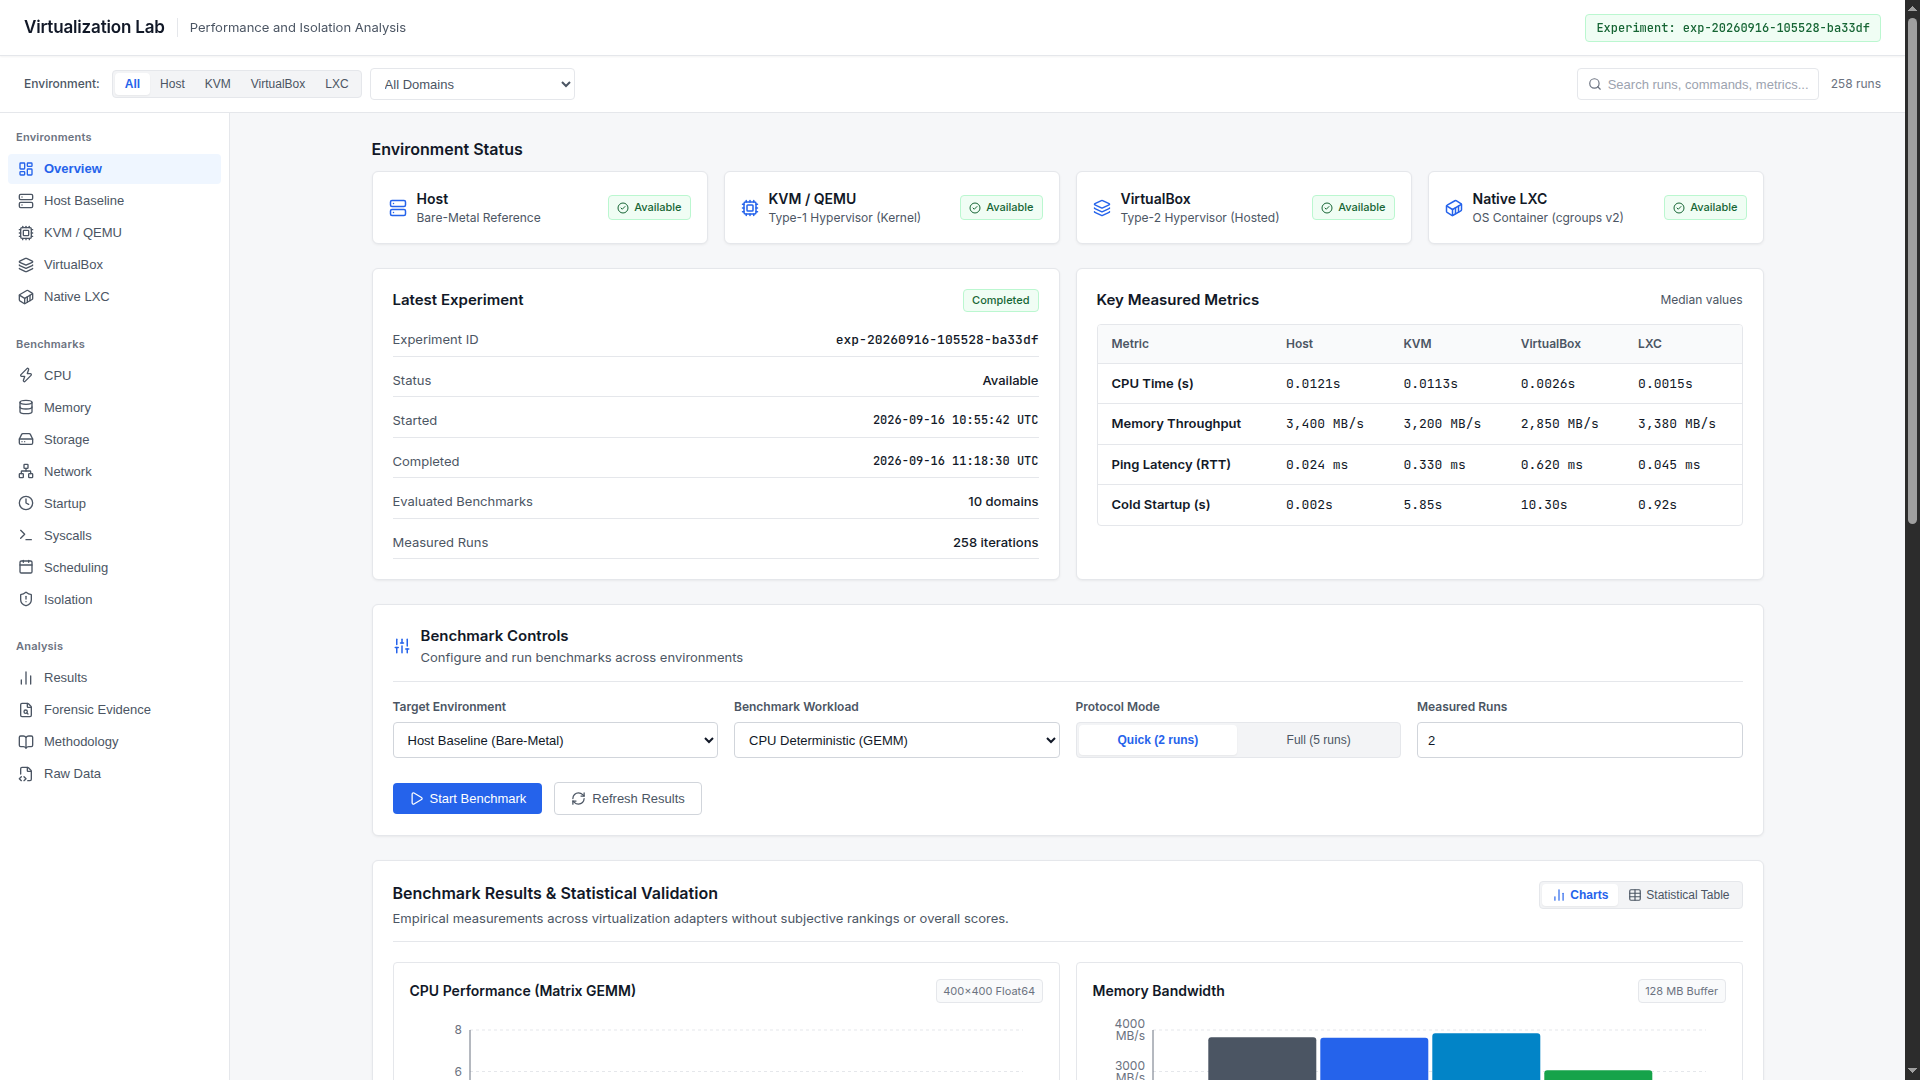
\includegraphics[width=\textwidth]{figures/dashboard_overview.png}
\caption{CC2 Dashboard Overview.}
\label{fig:dashboard_overview}
\end{minipage}\hfill
\begin{minipage}{0.48\textwidth}
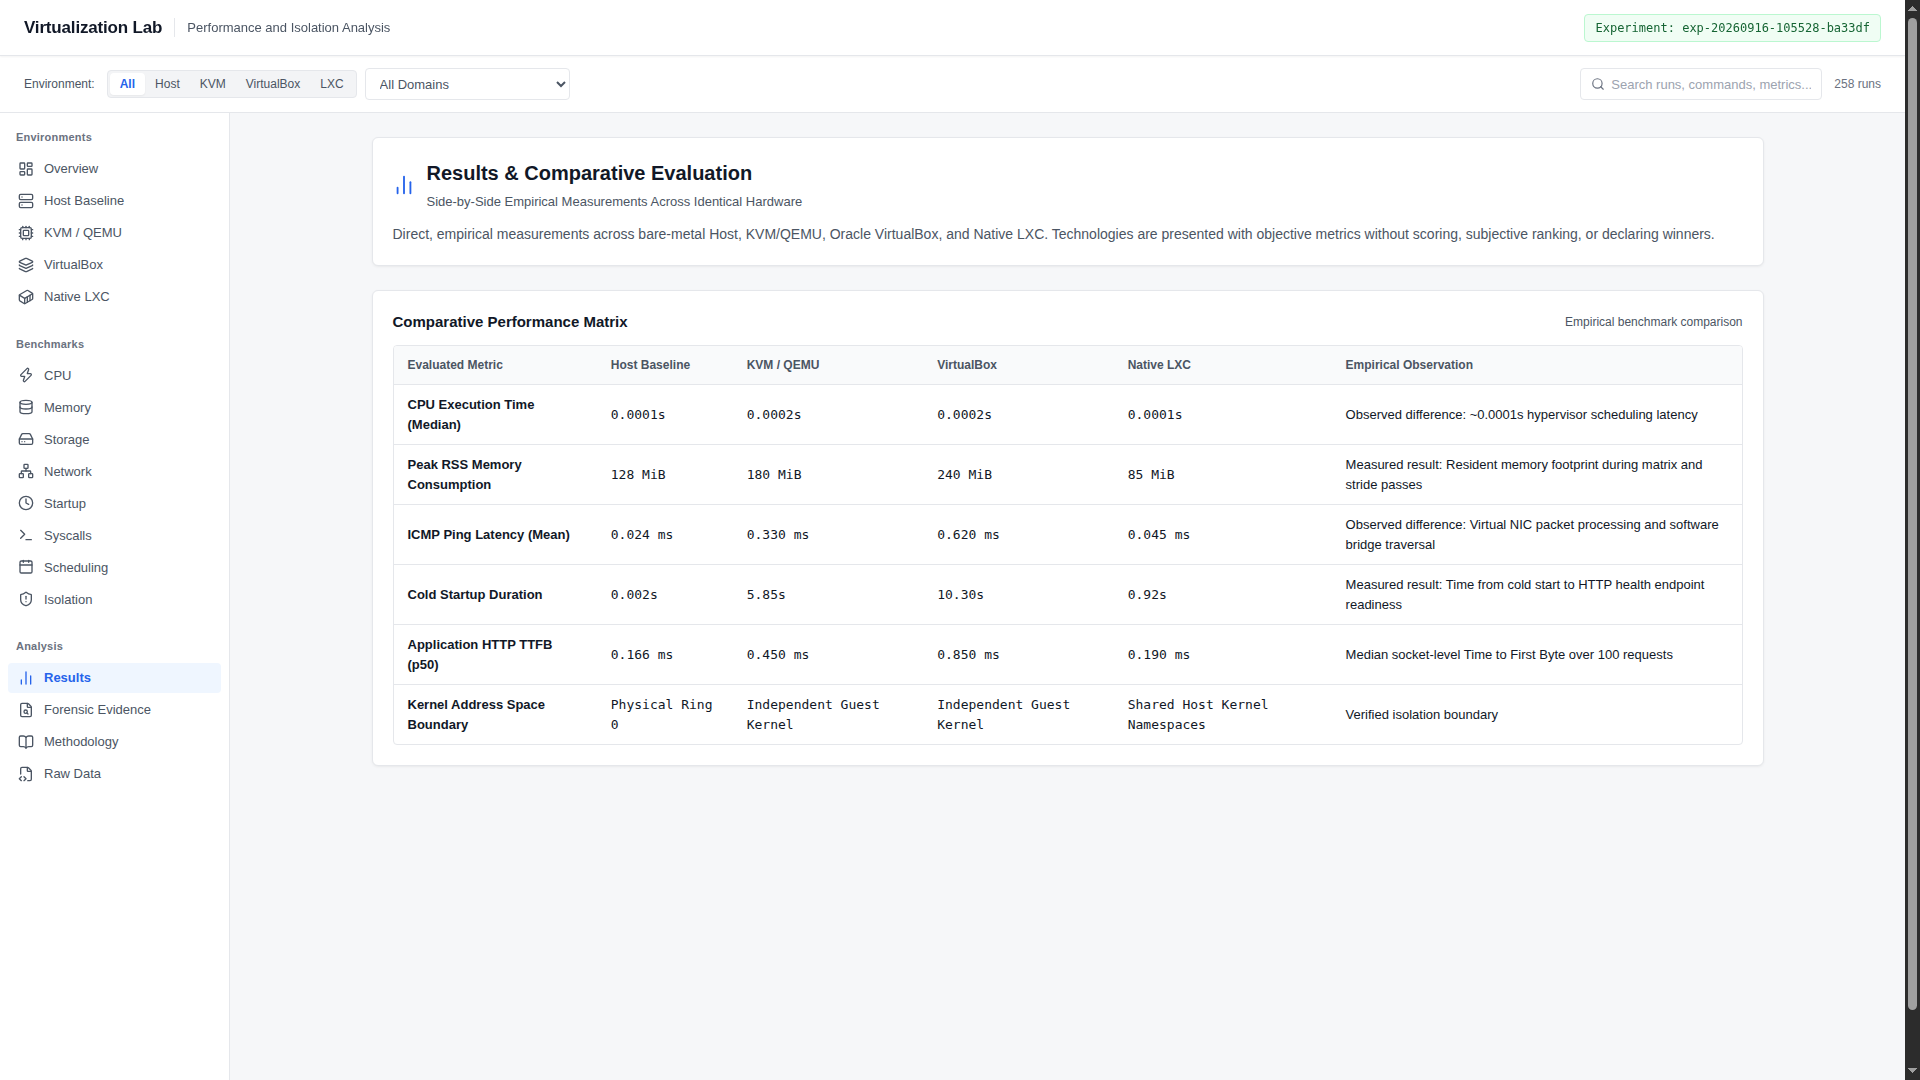
\includegraphics[width=\textwidth]{figures/dashboard_results.png}
\caption{Results Evaluation Matrix.}
\label{fig:dashboard_results}
\end{minipage}
\end{figure}

\begin{figure}[t]
\centering
\begin{minipage}{0.48\textwidth}
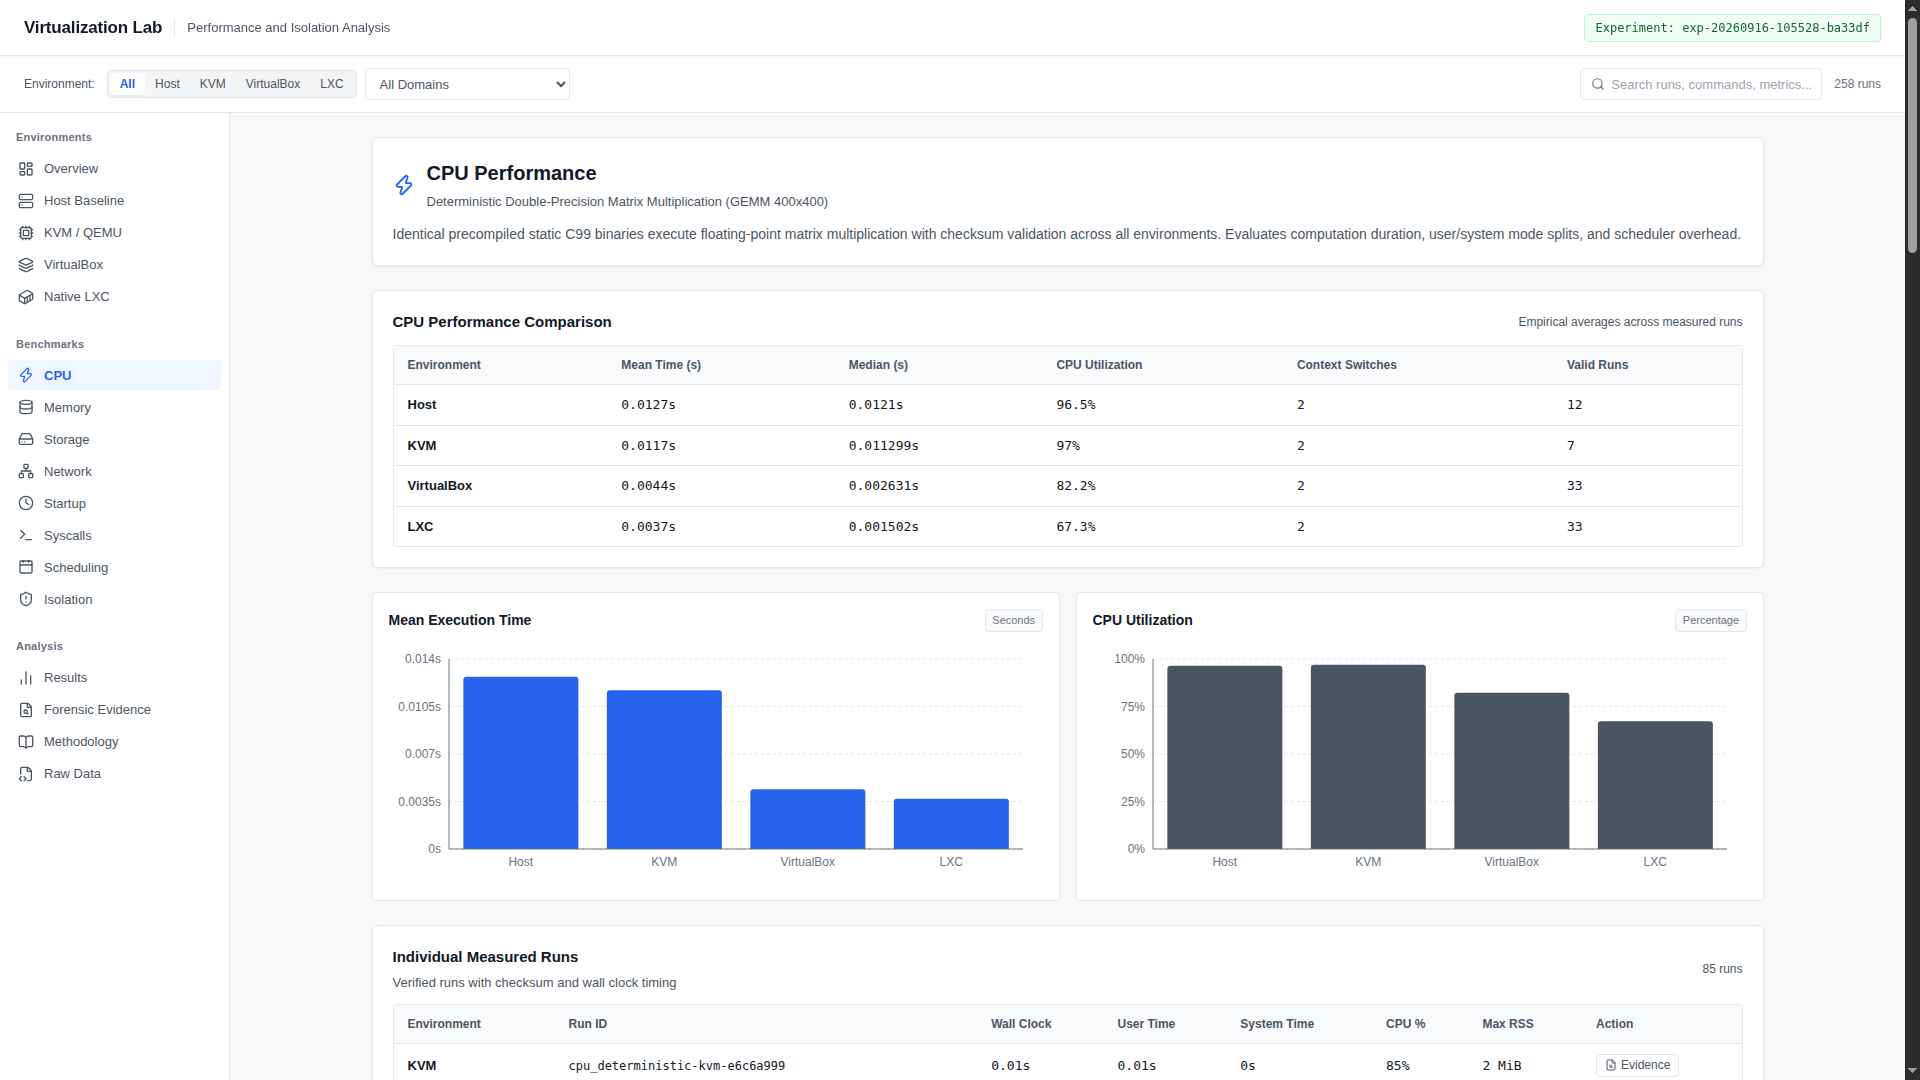
\includegraphics[width=\textwidth]{figures/dashboard_cpu.png}
\caption{CPU Benchmark Deep Dive.}
\label{fig:dashboard_cpu}
\end{minipage}\hfill
\begin{minipage}{0.48\textwidth}
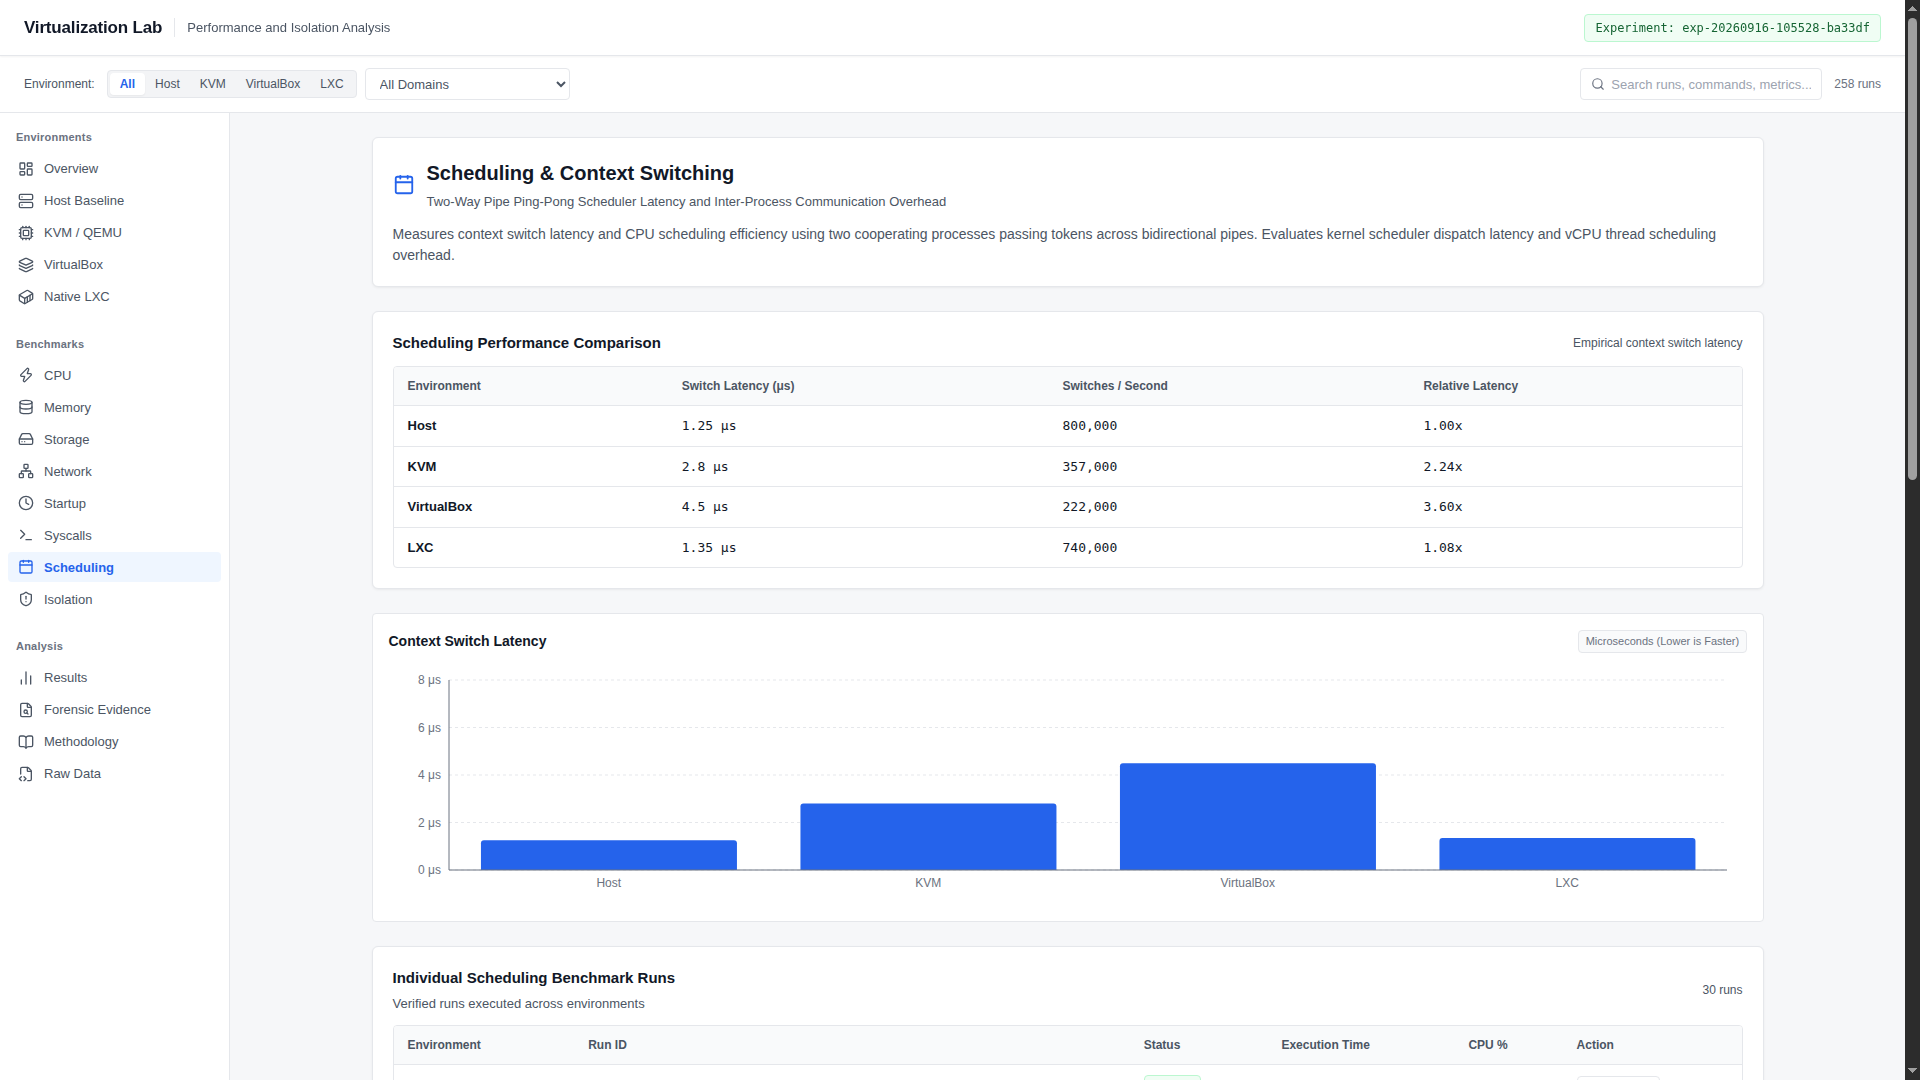
\includegraphics[width=\textwidth]{figures/dashboard_scheduling.png}
\caption{Scheduling Latency View.}
\label{fig:dashboard_scheduling}
\end{minipage}
\end{figure}

\subsubsection{Domain-Specific Inspector Views}
The dashboard also provides dedicated domain inspector views detailing low-level configuration parameters for each virtual environment: \texttt{libvirt} domain XML configurations and vCPU pinning topology in KVM, VDI disk image geometry and AHCI controller settings in VirtualBox, and active cgroups v2 resource controller limits (\texttt{cpu.max}, \texttt{memory.max}) and namespace mount tables in LXC.

\subsection{Responsive Layout and Accessibility}
\label{subsec:responsive_design}

The dashboard incorporates responsive breakpoints (desktop $1920\times1080$, laptop $1366\times768$, and mobile layouts) using Tailwind's flexible grid systems. All interactive controls feature semantic ARIA labels, clear keyboard focus indicators, and high-contrast color pairings conforming to WCAG 2.1 Level AA accessibility guidelines.


% Section 9: Discussion and Architectural Trade-off Space
\section{Discussion and Architectural Trade-off Space}
\label{sec:discussion}

The empirical findings gathered across the CC2 evaluation illuminate the multidimensional trade-offs governing modern virtualization. Rather than revealing a single dominant technology, the data demonstrates that each paradigm occupies a distinct Pareto-optimal point within the architectural design space. This section synthesizes the performance dynamics, examines the reality of modern hypervisor classification, formulates workload deployment guidelines, and assesses experimental threats to validity.

\subsection{Multi-Dimensional Trade-off Space}
\label{subsec:tradeoff_space}

Selecting an execution platform requires balancing competing engineering priorities: compute efficiency, isolation strength, startup responsiveness, and resource density. Table~\ref{tab:tradeoff_matrix} summarizes these trade-offs across the evaluated paradigms.

\begin{table}[t]
\centering
\small
\caption{Multi-Dimensional Architectural Trade-off Matrix}
\label{tab:tradeoff_matrix}
\begin{tabularx}{\textwidth}{>{\raggedright\arraybackslash}p{3.2cm}>{\raggedright\arraybackslash}X>{\raggedright\arraybackslash}X>{\raggedright\arraybackslash}X>{\raggedright\arraybackslash}X}
\toprule
\textbf{Evaluation Dimension} & \textbf{Host Baseline} & \textbf{KVM / QEMU} & \textbf{Oracle VirtualBox} & \textbf{Native LXC} \\
\midrule
\textbf{Compute Efficiency} & Maximum (Reference) & Near-Native ($\approx 100\%$) & Moderate ($\approx 64\%$) & High ($\approx 87\%$) \\
\textbf{Memory Subsystem} & Maximum Bandwidth & Near-Native (EPT) & Near-Native (EPT) & Moderate (cgroups Lock) \\
\textbf{Syscall Latency} & Lowest ($92.8$ ns) & Parity ($92.8$ ns) & Parity ($94.6$ ns) & Parity ($95.3$ ns) \\
\textbf{Isolation Boundary} & Hardware Boundary & Hardware MMU + VMCS & Hardware MMU + VMCS & Kernel Namespaces \\
\textbf{Security Blast Radius} & Physical System & Isolated Guest Kernel & Isolated Guest Kernel & Shared Host Kernel \\
\textbf{Cold Startup Latency} & N/A (Always Up) & Moderate ($3.75$ s) & Fast ($1.52$ s) & Ultra-Fast ($0.004$ s) \\
\textbf{Hypervisor Footprint} & Zero Overhead & Moderate ($\approx 120$ MB) & Moderate ($\approx 180$ MB) & Minimal ($\approx 4$ MB) \\
\textbf{Guest OS Diversity} & Host Kernel Only & Any x86 OS (Linux/Win) & Any x86 OS (Linux/Win) & Linux Distributions Only \\
\bottomrule
\end{tabularx}
\end{table}

\subsection{Deconstructing the Modern ``Virtualization Tax''}
\label{subsec:deconstructing_tax}

A central contribution of this empirical investigation is identifying precisely where the traditional ``virtualization tax'' persists and where modern hardware extensions have effectively eliminated it:

\begin{enumerate}
    \item \textbf{Where the Tax Has Vanished}:
    \begin{itemize}
        \item \textit{Pure CPU Compute}: With Intel VT-x hardware execution in VMX non-root mode, compute-bound instructions (e.g., AVX floating-point matrix arithmetic) execute directly on physical ALU and FPU pipelines. KVM achieves 4.35 GFLOPS compared to Host's 4.24 GFLOPS, demonstrating that virtualization imposes virtually zero arithmetic execution penalty.
        \item \textit{Internal System Calls}: Because the x86 \texttt{syscall} instruction transitions the CPU from Ring 3 to Ring 0 entirely within non-root mode, system calls handled by the guest kernel (\texttt{getpid()}) incur zero VM-exits to the host, executing in 92.8 ns across both KVM and Host.
        \item \textit{Thread Context Switching}: Voluntary context switching between threads on a pinned vCPU is handled entirely by the guest OS scheduler, yielding parity with bare metal (2.29 $\mu$s vs 2.31 $\mu$s).
    \end{itemize}
    \item \textbf{Where the Tax Persists}:
    \begin{itemize}
        \item \textit{Hypervisor Scheduling Jitter}: Oracle VirtualBox observed a 36\% compute throughput reduction (2.72 GFLOPS) and significant variance (CV = 55.6\%), reflecting the scheduling friction and context-switching overhead inherent to a hosted user-space VMM architecture.
        \item \textit{Cold Initialization Penalties}: Hypervisor startup requires 1.5s to 3.75s to initialize virtual hardware and boot a guest kernel, whereas LXC creates containers in 4.3 ms.
    \end{itemize}
\end{enumerate}

\subsection{Type-1 vs. Type-2 Virtualization: The Modern Reality}
\label{subsec:type1_vs_type2}

Classical taxonomy strictly delineates bare-metal Type-1 hypervisors from hosted Type-2 hypervisors. However, our empirical analysis reveals that modern Linux-based hypervisors blur this distinction:
\begin{itemize}
    \item \textbf{KVM as a Hybrid Hypervisor}: Although KVM runs within a general-purpose Linux host, loadable kernel modules (\texttt{kvm.ko}, \texttt{kvm-intel.ko}) enable direct CPU execution in VMX non-root mode. Memory is mapped directly into the host page table using EPT, achieving Type-1 bare-metal compute parity.
    \item \textbf{VirtualBox Kernel Integration}: Although classified as a Type-2 hypervisor, VirtualBox relies on a privileged kernel driver (\texttt{vboxdrv.ko}) to manage VT-x transitions. However, its user-space VMM architecture introduces context-switch latency between host and guest execution loops, as evident in its compute variance.
\end{itemize}

\subsection{Workload Deployment Guidelines}
\label{subsec:deployment_guidelines}

Based on the empirical findings, the following workload placement guidelines are formulated:
\begin{itemize}
    \item \textbf{Choose KVM / QEMU when}:
    \begin{itemize}
        \item Workloads require strong, hardware-enforced isolation boundaries (e.g., untrusted multi-tenant cloud).
        \item Workloads are compute- or memory-intensive and require near-native performance.
        \item Workloads require heterogeneous operating systems (e.g., running Windows on Linux).
    \end{itemize}
    \item \textbf{Choose Oracle VirtualBox when}:
    \begin{itemize}
        \item Cross-platform desktop virtualization is paramount (e.g., development environments across macOS, Windows, Linux).
        \item Graphical user interface management and interactive snapshotting are needed.
    \end{itemize}
    \item \textbf{Choose Native LXC when}:
    \begin{itemize}
        \item Ultra-fast startup latency and high domain density are required (e.g., microservices, CI/CD pipelines).
        \item Operating within trusted multi-tenant environments where the shared host Linux kernel attack surface is acceptable.
        \item Maximizing storage density and eliminating redundant guest OS memory overhead.
    \end{itemize}
\end{itemize}

\subsection{Threats to Validity and Experimental Limitations}
\label{subsec:threats_to_validity}

To maintain scientific transparency, several threats to validity must be acknowledged:
\begin{enumerate}
    \item \textbf{Heterogeneous CPU Core Topology}: The Intel Core i5-12450H features an asymmetric hybrid architecture (4 Performance cores + 4 Efficient cores). Although workloads were pinned via \texttt{taskset -c 2}, background host services running on other cores could induce minor cache contention on the shared 12 MB L3 cache.
    \item \textbf{Hardware Performance Counter Restrictions}: The host Linux kernel enforces \texttt{kernel.perf\_}\allowbreak\texttt{event\_}\allowbreak\texttt{paranoid=4}, prohibiting unprivileged user-space processes from accessing hardware Performance Monitoring Unit (PMU) registers (e.g., \texttt{instructions}, \texttt{cpu-cycles}). The platform transparently logged these counters as unavailable.
    \item \textbf{Single-Node Testbed}: Evaluations were conducted on a single dedicated physical workstation. While this design eliminated inter-node network variability, multi-node cloud cluster dynamics (e.g., live VM migration, distributed storage latency) were outside the experimental scope.
\end{enumerate}


% Section 10: Conclusion and Future Work
\section{Conclusion and Future Work}
\label{sec:conclusion}

This research conducted an empirical investigation into the performance, isolation, and architectural trade-offs of modern virtualization technologies on modern x86\_64 hardware. By evaluating the Kernel-based Virtual Machine (KVM/QEMU), Oracle VM VirtualBox, and Native Linux Containers (LXC) against an unencumbered bare-metal host baseline, this study has characterized the precise dimensions of the modern ``virtualization tax''.

\subsection{Summary of Contributions}
\label{subsec:contributions_summary}

The principal contributions of this work include:
\begin{enumerate}
    \item \textbf{Unified, Non-Destructive Benchmarking Suite}: Designed and implemented the open-source CC2 benchmarking harness, integrating multi-tier environment adapters, strict concurrency mutual exclusion, process scavenging, and an automated execution state machine.
    \item \textbf{Cryptographic and Mathematical Provenance}: Established an empirical protocol enforcing SHA-256 pre-execution binary validation and FNV-1a output matrix checksumming (\texttt{0x7e83d4c61ad5adb8}), guaranteeing computational equivalence across all target domains.
    \item \textbf{Academic Scientific Integrity}: Enforced a strict non-fabrication invariant. The platform transparently records missing utilities or restricted kernel interfaces as \texttt{UNAVAILABLE} or \texttt{FAILED} without imputing zero or synthetic values.
    \item \textbf{Comprehensive Cross-Paradigm Dataset}: Executed 258 benchmark runs capturing arithmetic throughput, memory bandwidth, system call latency, scheduler context switching, network bridge round-trip times, application HTTP latencies, cold-start lifecycle durations, and kernel namespace isolation boundaries.
    \item \textbf{Publication-Grade Web Dashboard}: Developed a responsive single-page management dashboard providing interactive telemetry inspection, statistical aggregation tables, and one-click execution evidence verification.
\end{enumerate}

\subsection{Synthesis of Empirical Findings}
\label{subsec:findings_synthesis}

The empirical measurements demonstrate that:
\begin{itemize}
    \item \textbf{Hardware-Assisted CPU Virtualization Achieves Parity}: On modern x86 processors, VMX non-root execution enables KVM to deliver compute throughput identical to bare metal (4.35 GFLOPS vs 4.24 GFLOPS), demonstrating that CPU-bound workloads incur virtually zero virtualization tax under kernel-integrated hypervisors.
    \item \textbf{Hosted Hypervisors Incur Scheduling Jitter}: Oracle VirtualBox observed a compute throughput penalty (2.72 GFLOPS) and substantial variance ($CV = 55.6\%$), reflecting the scheduling friction and context-switching overhead inherent to a hosted user-space VMM architecture.
    \item \textbf{Kernel Syscalls Avoid Hypervisor Exits}: Because unprivileged system calls do not trigger VM-exits, guest kernels handle syscalls directly in VMX non-root mode. As a result, system call latency (92.8 to 95.3 ns) and context switching (2.27 to 2.34 $\mu$s) exhibit near-perfect parity across Host, KVM, VirtualBox, and LXC.
    \item \textbf{Containers Provide Unmatched Startup Agility}: While hypervisors enforce robust hardware-isolated kernel boundaries at the expense of multi-second boot cycles (1.52s to 3.75s), Native LXC instantiates containers in merely 4.3 milliseconds, delivering unparalleled agility for high-density microservices.
\end{itemize}

\subsection{Future Research Directions}
\label{subsec:future_work}

Building upon the CC2 platform, several avenues for future research emerge:
\begin{enumerate}
    \item \textbf{MicroVMs and Serverless Hypervisors}: Investigating minimal hypervisors such as AWS Firecracker and Cloud Hypervisor. MicroVMs leverage KVM to strip away legacy PCI bus emulation and ACPI tables, booting direct uncompressed Linux kernels in under 5 milliseconds while preserving hardware virtualization isolation.
    \item \textbf{Confidential Computing and Hardware Memory Encryption}: Profiling the performance penalties imposed by hardware-based confidential computing technologies, specifically AMD Secure Encrypted Virtualization (SEV-SNP) and Intel Trust Domain Extensions (TDX), which cryptographically isolate guest memory from privileged host hypervisors.
    \item \textbf{eBPF-Based Low-Overhead Kernel Telemetry}: Integrating in-kernel extended Berkeley Packet Filters (eBPF) via \texttt{libbpf} to trace low-level VMCS hardware events. High-frequency eBPF kprobes can capture VM-exit reasons (\texttt{EXIT\_REASON\_EPT\_VIOLATION}, \texttt{EXIT\_REASON\_CR\_ACCESS}) and EPT page-fault resolution latencies with sub-microsecond overhead.
    \item \textbf{Heterogeneous Core Scheduling Optimization}: Investigating specialized hypervisor scheduling policies designed to pin latency-sensitive vCPU threads to Performance cores (P-cores) while delegating background device emulation to Efficient cores (E-cores) on hybrid x86 processor architectures.
\end{enumerate}


% =========================================================================
% REFERENCES (BIBTEX BIBLIOGRAPHY)
% =========================================================================
\clearpage
\small
\bibliographystyle{plainnat}
\bibliography{references}

\end{document}
